% Paper: learned layers on top of the factor pipeline (what worked, what did not, why).

% ---- begin ../shared/docclass.tex
% Document class selection (\input as the first line of each main.tex).
% SIMODS is typeset with SIAM's online-journal class siamonline<date>.cls. The class is not on CTAN;
% download it from SIAM's author page (the CI tries to) and place it in paper/shared/siam/.
% Without it the paper builds with a compatible fallback (article + siamshim.tex), so that text,
% numbering and cross-references can be checked; the submission must use the official class.
\makeatletter
\let\pf@cls\relax
\IfFileExists{siamonline220329.cls}{\def\pf@cls{siamonline220329}}{}
\IfFileExists{siamonline250211.cls}{\def\pf@cls{siamonline250211}}{}
\ifx\pf@cls\relax
  \documentclass[11pt]{article}
  \def\paperclass{shim}
\else
  \edef\pf@doc{\noexpand\documentclass[review,onefignum,onetabnum]{\pf@cls}}
  \pf@doc
  \def\paperclass{siam}
\fi
\makeatother

% ---- end ../shared/docclass.tex


% ---- begin ../shared/preamble.tex
% Common preamble of both papers (after docclass.tex).
\def\pfshimname{shim}
\ifx\paperclass\pfshimname
  
% ---- begin ../shared/siamshim.tex
% Fallback that mimics the parts of siamonline used by the papers (only when the class is absent).
\usepackage[letterpaper,margin=1.15in]{geometry}
\usepackage{amsmath,amssymb,amsthm}
\usepackage[T1]{fontenc}
\usepackage{lmodern}
\usepackage{fancyhdr}
\newcommand{\headers}[2]{\pagestyle{fancy}\fancyhf{}\fancyhead[LE]{\small\thepage\quad\textsc{#2}}%
  \fancyhead[RO]{\small\textsc{#1}\quad\thepage}\fancyhead[LO,RE]{}\renewcommand{\headrulewidth}{0pt}}
\newcommand{\email}[1]{\texttt{#1}}
\newcommand{\funding}[1]{\par\noindent\textbf{Funding:} #1}
\newenvironment{keywords}{\par\smallskip\noindent\textbf{Key words.}\ }{\par}
\newenvironment{MSCcodes}{\par\smallskip\noindent\textbf{MSC codes.}\ }{\par}
\newenvironment{AMS}{\par\smallskip\noindent\textbf{AMS subject classifications.}\ }{\par}
\renewenvironment{abstract}{\par\small\noindent\textbf{Abstract.}\ }{\par\normalsize}

% ---- end ../shared/siamshim.tex

\else
  \usepackage{amssymb}
  \newsiamremark{remark}{Remark}
  \newsiamremark{example}{Example}
  \newsiamthm{assumption}{Assumption}
\fi
\usepackage{mathtools}
\usepackage{graphicx}
\graphicspath{{../shared/figures/}}
\usepackage{booktabs,array,tabularx,multirow}
\usepackage[dvipsnames]{xcolor}
\usepackage{tikz}
\usetikzlibrary{arrows.meta,positioning,calc,fit,shapes.geometric,backgrounds}
\usepackage{algorithm}
\usepackage{algpseudocode}
\usepackage{enumitem}
\setlist{nosep,leftmargin=*}
\ifx\paperclass\pfshimname
  \usepackage[hidelinks]{hyperref}
  \usepackage[capitalize,nameinlink]{cleveref}
  
% ---- begin ../shared/siamshim_thm.tex
% Fallback theorem environments (loaded after hyperref and cleveref so that names resolve).
\theoremstyle{plain}
\newtheorem{theorem}{Theorem}[section]
\newtheorem{lemma}[theorem]{Lemma}
\newtheorem{proposition}[theorem]{Proposition}
\newtheorem{corollary}[theorem]{Corollary}
\theoremstyle{definition}
\newtheorem{definition}[theorem]{Definition}
\newtheorem{assumption}[theorem]{Assumption}
\theoremstyle{remark}
\newtheorem{remark}[theorem]{Remark}
\newtheorem{example}[theorem]{Example}

% ---- end ../shared/siamshim_thm.tex

\else
  \makeatletter\@ifpackageloaded{cleveref}{}{\usepackage[capitalize,nameinlink]{cleveref}}\makeatother
\fi
\crefname{assumption}{Assumption}{Assumptions}
\crefname{example}{Example}{Examples}
\crefname{remark}{Remark}{Remarks}
\crefname{algorithm}{Algorithm}{Algorithms}

% ---- begin ../shared/macros.tex
% ---------------------------------------------------------------------------------------------
% Notation macros. ONE symbol, ONE meaning: every macro below is listed in the notation table
% (sections/notation.tex) and the script tools/check_notation.py checks the correspondence.
% ---------------------------------------------------------------------------------------------
% number sets and rings
\newcommand{\R}{\mathbb{R}}
\newcommand{\C}{\mathbb{C}}
\newcommand{\Z}{\mathbb{Z}}
\newcommand{\ring}{\mathcal{R}}            % ring of constant-coefficient operators C[d_t,d_x] = C[tau,xi]
% operators and their algebra
\DeclareMathOperator{\Ann}{Ann}             % annihilator ideal of a function
\DeclareMathOperator{\gcdop}{gcd}
\DeclareMathOperator{\spn}{span}
\DeclareMathOperator{\rank}{rank}
\DeclareMathOperator{\diag}{diag}
\DeclareMathOperator{\tr}{tr}
\newcommand{\Var}{V}                        % characteristic variety V(P)
\newcommand{\EP}{\mathrm{EP}}               % exponential-polynomials
\newcommand{\dd}{\,\mathrm{d}}
\newcommand{\Id}{\mathrm{Id}}
\newcommand{\Gu}{G_u}                       % intrinsic operator gcd Ann(u)
\newcommand{\Ju}{J_u}                       % cofactor ideal, Ann(u) = G_u J_u
\newcommand{\sigp}{\Sigma_{\mathrm p}}      % point spectrum V(J_u)
\newcommand{\sumop}{\mathcal{S}}            % sum operator (u_1,...,u_N) -> sum u_j
\newcommand{\Eint}{E_{\mathrm{int}}}        % interaction term
\newcommand{\flow}{\Phi}                    % flows Phi_n(t) = e^{t A_n}
\newcommand{\cF}{c_{F}}                     % Friedrichs cosine
\newcommand{\thetaF}{\theta_{F}}            % Friedrichs angle
\newcommand{\gN}{\gamma_{N}}                % conditioning constant of the sum operator
\newcommand{\deltaP}{\delta(P)}             % ambiguity dimension
\newcommand{\Hs}{H^{s}}                     % Sobolev space of index s
\newcommand{\noise}{\sigma_{n}}             % observation noise standard deviation
\newcommand{\sigbin}{\sigma_{\kappa}}       % noise standard deviation of one Fourier bin
\newcommand{\Nsamp}{N_{\mathrm s}}          % number of posterior field samples
\newcommand{\keff}{k_{\mathrm{eff}}}        % effective number of factors
\newcommand{\cloud}{W}                      % cloud of factor vectors (a weighted point measure)
\newcommand{\Mfit}{\mathsf{M}}              % a candidate structure (model)
\newcommand{\lab}[1]{\textsf{#1}}           % output labels
\newcommand{\FC}{\lab{FIT-COMPATIBLE}}
\newcommand{\IDK}{\lab{ID-KER}}
\newcommand{\MIS}{\lab{MISFIT}}
\newcommand{\UND}{\lab{UNDECIDED}}
\newcommand{\Normal}{\mathcal{N}}
\newcommand{\E}{\mathbb{E}}
\newcommand{\abs}[1]{\lvert#1\rvert}
\newcommand{\norm}[1]{\lVert#1\rVert}
\newcommand{\ip}[2]{\langle#1,#2\rangle}
% editorial
\newcommand{\roleinalg}[1]{\par\noindent\emph{Role in the algorithm.} #1\par}
\newcommand{\inbrief}[1]{\par\smallskip\noindent\emph{In brief.} #1\par\smallskip}

% ---- end ../shared/macros.tex


% ---- end ../shared/preamble.tex

\usepackage{longtable}
% macros of the explained edition
\usepackage{caption,needspace}
\definecolor{cA}{HTML}{1F4E79}\definecolor{cB}{HTML}{C0392B}\definecolor{cC}{HTML}{1E8449}\definecolor{cD}{HTML}{B9770E}\definecolor{cG}{HTML}{7F8C8D}
\newcolumntype{L}[1]{>{\raggedright\arraybackslash}p{#1}}
\newcommand{\badge}[2]{\textcolor{#1}{\textsf{\footnotesize[#2]}}}
\newcommand{\impl}{\badge{cC}{implemented, tested}}
\newcommand{\implu}{\badge{cD}{implemented, uncommitted}}
\newcommand{\proto}{\badge{cD}{prototype}}
\newcommand{\plan}{\badge{cB}{planned}}
\newcommand{\openq}{\badge{cB}{open}}
\newcommand{\thy}[1]{\textcolor{cG}{\textsf{\footnotesize(theory #1)}}}
\newcommand{\sectionbrief}[3]{\par\noindent{\small\emph{In this section.} #1 #2 #3}\par\smallskip}
\newenvironment{capbox}[1]{\begin{remark}[#1]}{\end{remark}}
\newenvironment{intuition}[1][]{\begin{remark}[Intuition]}{\end{remark}}
\newenvironment{caution}[1][]{\begin{remark}[Warning]}{\end{remark}}
\newenvironment{takeaway}{\begin{remark}[Why it matters]}{\end{remark}}
\newenvironment{keypoint}{\begin{remark}[Takeaway]}{\end{remark}}
\newenvironment{notebox}[1]{\begin{remark}[#1]}{\end{remark}}
\newenvironment{aside}[1]{\begin{remark}[#1]}{\end{remark}}
\newenvironment{explained}[1]{\begin{remark}[Explained: #1]}{\end{remark}}
\newenvironment{wstep}[1]{\par\medskip\noindent\textbf{#1}\par\nopagebreak}{\par\medskip}
\newenvironment{ideabox}[1][]{\begin{remark}[Idea]}{\end{remark}}
\newenvironment{askbox}[1]{\begin{remark}[#1]}{\end{remark}}
\newenvironment{iobox}[1]{\begin{remark}[#1]}{\end{remark}}
\newenvironment{symbols}{\begin{remark}[Symbols used here]}{\end{remark}}

\title{Learned Layers for a Factor-Based PDE Pipeline:\\What Worked, What Did Not, and Why}
\author{Flavio Pricoco\thanks{\email{flaflapr@gmail.com}}}
\headers{Learned layers for a factor-based PDE pipeline}{F. Pricoco}

\begin{document}
\maketitle

\begin{abstract}
A pipeline that reads the factors of a linear partial differential equation from noisy data already contains classical
statistical learning: a Gaussian process interpolates, a Dirichlet-process mixture groups, a Bayesian linear model splits
components. This paper asks a different question: can \emph{learned} layers, trained on simulated equations, make that
pipeline more accurate, better calibrated or faster, without ever changing what it is allowed to claim? We state a
contract under which a learned layer may propose a candidate, fit a global constant, or raise a flag, but never decide a
label, and under which every layer switched off reproduces the pipeline bit for bit. We designed eight such layers, built seven, and
gated each on held-out equation families, with leave-one-family-out validation, paired cluster bootstrap and conformal
operating points. One layer ships: an exact memo that is bit-identical to the pipeline and saves about half a percent of the time.
A learned failure detector separates injected failures from clean runs (cross-validated AUROC $0.85$, against $0.63$ for the
pipeline's own omnibus test) but has almost no detection power at the $5\%$ false-alarm level it needs, and a
controller that reruns the pipeline with other settings has an oracle ceiling of $8$ of $12$ failures, reduced to $0$ of $12$
once a real trigger is required. The calibration layers fail because the quantity they would calibrate is saturated
or already calibrated. We report each negative result with its numbers, the lessons they share, and the ideas that remain.
\end{abstract}

\begin{keywords}
equation discovery, uncertainty calibration, conformal prediction, failure detection, negative results
\end{keywords}

\begin{MSCcodes}
35E20, 62F15, 62G15, 68T05
\end{MSCcodes}

\section{Introduction}\label{sec:intro}
The pipeline studied here takes noisy observations of a field $u(t,x)$ that solves a linear constant-coefficient equation
and returns a distribution over equations, each with intervals on its coefficients and one of four labels: \FC, \MIS,
\IDK, \UND{}. It never prints that a law is identified. Its design and the mathematics behind it are in the companion
papers; here we only need its behaviour. On a development benchmark it is right on all thirty inputs and never wrong
without warning. On twenty random equations it returns the right or an equivalent equation on nineteen. Yet on a larger
simulated corpus of random equations from five families, on the earlier pipeline version the layers were built on and with every learned layer off, it is \emph{false-confident} on
$9$ of $80$ held-out grid cases: it reports \FC{} for a wrong factor set.

That figure is the motivation. Is there a learned component, trained on simulated equations, that removes such errors,
or that tells us when they occur? The question matters beyond this pipeline, because learned correction layers are
the usual answer to residual miscalibration in scientific methods, and rarely come with a pre-registered gate and a
report of the layers that failed it.

\paragraph{What we did} We defined a contract for learned layers (\cref{sec:contract}), built the layers the pipeline
admits (\cref{sec:pipeline}), and evaluated each against a gate fixed before the run, on corpora of simulated equations that
do not overlap the development benchmark (\cref{sec:protocol}).

\paragraph{What we found} Of eight layers (seven built), one is on by default and it is a pure speed-up (\cref{sec:worked}). A learned
failure detector is the only layer with a positive effect on the quantity it targets, and that effect does not survive the
operating point the contract requires (\cref{sec:v1}). The others are negative: a learned skip of optional steps saves
at most $0.7\%$ of the time (\cref{sec:lb}); calibration of interval widths and of the top-structure probability does not
help (\cref{sec:calib}); a scan for high wavenumbers never changes an answer (\cref{sec:highk}); a controller that
chooses reruns has an upper bound that no available trigger reaches (\cref{sec:controller}). \Cref{tab:verdicts} lists all
verdicts. \Cref{sec:lessons} extracts what the failures have in common, and \cref{sec:ideas} lists ideas not yet tried,
including the author's own.

\paragraph{Structure} \Cref{sec:pipeline,sec:inside-ml} describe the pipeline and the statistical learning already inside it; \cref{sec:contract,sec:protocol,sec:p0} give the contract, the protocol and the prerequisites; \cref{sec:design} states every layer as designed, built or not;
\cref{sec:worked,sec:v1,sec:negative} report what was built and what happened, including the controller in detail (\cref{sec:controller-built}) and what was never built (\cref{sec:unbuilt}); the appendices hold the failure-mode table, the acceptance protocol and the test inventory.

\paragraph{Scope} Everything here concerns linear, constant-coefficient, autonomous, scalar equations in one space and one
time variable. The layers were developed on one version of the pipeline (\cref{sec:repro}); we say so wherever it matters.

\section{The pipeline and where learning can enter}\label{sec:pipeline}
\Cref{fig:layers} shows the pipeline as a chain of five steps and the places where a learned layer can attach.
\begin{figure}[tbp]
\centering
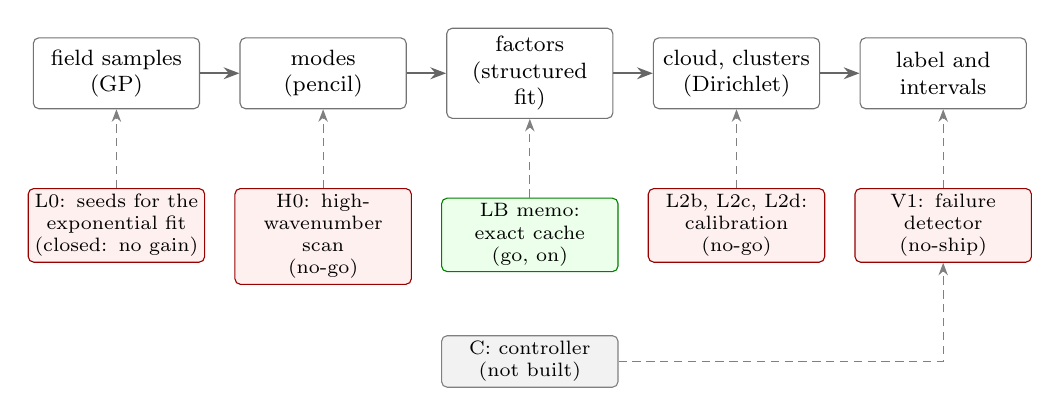
\begin{tikzpicture}[
  node distance=3mm and 5mm,
  box/.style={draw=black!55, rounded corners=2pt, align=center, font=\footnotesize, inner sep=3pt, minimum height=9mm, text width=19mm, fill=white},
  ok/.style={draw=green!50!black, fill=green!8, rounded corners=2pt, align=center, font=\scriptsize, inner sep=2pt, text width=21mm},
  no/.style={draw=red!60!black, fill=red!6, rounded corners=2pt, align=center, font=\scriptsize, inner sep=2pt, text width=21mm},
  un/.style={draw=black!50, fill=black!5, rounded corners=2pt, align=center, font=\scriptsize, inner sep=2pt, text width=21mm},
  arr/.style={-{Stealth[length=2mm]}, black!60, thick},
  dsh/.style={-{Stealth[length=1.6mm]}, black!50, densely dashed}]
\node[box] (a) {field samples\\(GP)};
\node[box, right=of a] (b) {modes\\(pencil)};
\node[box, right=of b] (c) {factors\\(structured fit)};
\node[box, right=of c] (d) {cloud, clusters\\(Dirichlet)};
\node[box, right=of d] (e) {label and\\intervals};
\draw[arr] (a)--(b); \draw[arr] (b)--(c); \draw[arr] (c)--(d); \draw[arr] (d)--(e);
\node[no, below=10mm of a] (l0) {L0: seeds for the exponential fit\\(closed: no gain)};
\node[no, below=10mm of b] (h0) {H0: high-wavenumber scan\\(no-go)};
\node[ok, below=10mm of c] (lb) {LB memo: exact cache\\(go, on)};
\node[no, below=10mm of d] (l2) {L2b, L2c, L2d: calibration\\(no-go)};
\node[no, below=10mm of e] (v1) {V1: failure detector\\(no-ship)};
\node[un, below=8mm of lb] (c1) {C: controller\\(not built)};
\draw[dsh] (l0)--(a); \draw[dsh] (h0)--(b); \draw[dsh] (lb)--(c); \draw[dsh] (l2)--(d); \draw[dsh] (v1)--(e);
\draw[dsh] (c1.east) -| (v1.south);
\end{tikzpicture}
\caption{The pipeline (top) and the learned layers attached to it (below). Green: shipped; red: gated and rejected;
grey: designed, not built. Dashed arrows show the step each layer touches. V1 only reports; C would have used V1 as its
trigger.}\label{fig:layers}
\end{figure}

\paragraph{Learning already inside the pipeline} Three components are statistical learning and are part of the pipeline,
not optional layers: a Gaussian process (with scalable variants) that interpolates scattered data into samples of the field
\cite{RasWil06}; a Dirichlet-process mixture over the factors of the posterior samples; and a Bayesian linear model that
splits the field into one component per factor. They are described and benchmarked in the companion papers. They are
fixed here.

\paragraph{The layers} Optional layers attach at the places in \cref{fig:layers}. L0 proposes starting values for the
exponential fit that extracts modes. H0 scans the raw residual for wavenumbers the Gaussian-process path misses. LB caches
repeated mode extractions (exact) or learns to skip optional steps. L2b, L2c and L2d calibrate, respectively, the
probability of the top structure, the interval widths, and the global constants of the decision rules. V1 predicts from the
pipeline's own output whether the answer is wrong. C would read V1 and rerun the pipeline with other settings.


% ---- begin sections/s_inside.tex
% Added section: the statistical learning that is part of the pipeline itself.
\section{Machine learning inside the pipeline}\label{sec:inside-ml}
Before the optional layers, four components of the pipeline are themselves statistical learning. They are committed, tested and benchmarked, and the optional layers of \cref{sec:design} sit on top of them.

\subsection{The Gaussian process: interpolation with probabilities}\label{sec:gp}
The core needs a field on a grid with an error model, and the data are scattered and noisy. A Gaussian process with a sum of separable kernels $k_t\otimes k_x$ (optionally with a time envelope that mimics $e^{\lambda t}$)
gives many plausible fields $\hat u_s$ with weights $\pi_s$ instead of one smooth curve \cite{RasWil06}. Hyperparameters, noise included, are marginalised: type-II maximum a posteriori, a Laplace approximation and importance reweighting by default,
NUTS for small samples, a random subset for large ones; samples come from pathwise conditioning (Matheron's rule). Alongside it: a factor-wise EPGP (features $e^{\lambda(\kappa)t+i\kappa x}$ on the factors' varieties, closed-form evidence),
KISS-GP on a grid (experimental, not calibrated), a deep ensemble (ablation, known to be under-dispersed away from the data), and a bridge that runs the core on the samples.
\emph{Tests} ($11$ in \texttt{test\_interp.py}): shapes and weights, loose coverage, samples matching the marginals, the subset path for large $n$, the mixture probability-integral transform against SciPy, the core bridge on transport plus diffusion,
EPGP prior draws solving transport, EPGP features on the variety, ensemble smoke test.
\emph{Coverage experiment}: nine named cases, $n\in\{400,2000\}$, noise $1\%$ and $5\%$, $54$ fits; the $90\%$ band covers $0.93, 0.92, 0.90, 0.89$ in the four cells and the median estimated noise is within $4\%$ of the true one; the criterion ($\pm5$ points at $50,90,95\%$) holds in $11$ of $12$ cells, the miss is conservative.
An RBF-only family set fails at $n=2000$ (coverage $0.84$--$0.86$): evidence prefers the smoothest kernel that fits and is overconfident, so the \emph{set} of kernel families is a prior choice made by calibration.
The first end-to-end test gave only $0.40$ weight to the right factors because the core assumed white noise; this led to per-bin correlated noise in the core.

\subsection{The Dirichlet-process mixture and clustering}\label{sec:dp}
The factors of all posterior samples form a weighted cloud $\cloud$. A truncated stick-breaking Dirichlet-process mixture is fitted per $\tau$-degree (scikit-learn's Bayesian Gaussian mixture) with a merge step by BIC for clusters that never co-occur in a sample;
the concentration is chosen by the variational bound and the effective number of factors is $\keff=\exp$ of the entropy of the masses. A second module extracts analytic window features and clusters rectangles by four methods (Gaussian mixture, $k$-means, spectral with adjacency, agglomerative with connectivity),
the number of groups being the MAP of a BIC posterior; a dominant-balance baseline is included. \emph{Tests} ($11$ in \texttt{test\_aggregate\_cluster.py}): invariance to padding and to factor order, aggregates of transport plus diffusion and of heat, rectangles and adjacency, the two-regime ARI for each method, the dominant-balance baseline.
\emph{Results}: $P(k=2)=1.0$ on transport plus diffusion with masses $(0.768,0.232)$; $P(k=1)=1.0$ on heat after the merge step (margin $7.96$ against $8.32$, thin); ARI $=1.0$ for all four methods when the windows are aligned with the regime boundary and $0.63$ for three of them when one straddles it; dominant balance $0.20$--$0.35$.
These runs used the exact components as input, so they show the method on clean separation only.

\subsection{The Bayesian split layer}\label{sec:split}
A linear-Gaussian model per Fourier bin gives credible intervals for the component weights (by Monte Carlo) and the probability that the split exists, with a real (conjugate-pair) parametrisation at $\kappa=0$ and a per-bin correlated noise covariance from the interpolation draws.
The same machinery supplies the \emph{raw evidence}, the Gaussian evidence of the raw scattered observations in the span of the factors' kernels, which the loop uses to choose the structure. \emph{Tests} ($10$ in \texttt{test\_phase3.py}): per-bin noise recovers an AR(1) autocovariance,
generalised least squares with white draws equals the white core, the weights cover the truth and the null stays low, the decider rejects constant factors per $\kappa$, rejects a symbol that interpolates few modes, counts only observed branches, rejects an interpolation artefact, and merges conjugate pairs.
\emph{Experiment}: noise $10^{-2}$, true factors; transport plus diffusion: $90\%$ interval coverage $0.95$--$1.00$ for $T\in[0.25,2]$; wave $0.85$--$1.00$; null (heat with a spurious transport) $P(\text{split})=0.000$. The first version covered only $0.65$--$0.85$, which led to the conjugate-pair parametrisation.

\subsection{The decider, the refinement and the loop}\label{sec:decider}
The loop chooses the structure by raw-data evidence with an Occam term and an outlier-bin mixture, refits the coefficients to the observations by variable projection with terms selected by evidence minus $\tfrac12p\log n$, splits reducible quadratics and conjugate pairs,
and grows the degree only under a held-out guard. \emph{Benchmark}: ten named cases $\times$ noise $\{10^{-3},10^{-2},5\cdot10^{-2}\}\times$ sampling $\{$grid, 2000, 400$\}$, $30$ runs per cell, against PDE-FIND, weak SINDy, ensemble SINDy, Bayesian SINDy and BOP-DMD:
right factor set on a grid $1.00/1.00/0.93$, with $2000$ points $1.00/0.97/0.90$, with $400$ points $1.00/0.93/0.73$, at least as good as every baseline in all nine cells; coefficient cover$_{90}$ $0.75$--$0.93$, weight cover$_{90}$ $0.50$--$1.00$.
\emph{Held-out equations}: random equations by family, $13$ draws, right or equivalent on $10$, one correct abstention, no false-confident answer.
\emph{What this part does not show}: the ten named cases both tuned and measured the defaults; the hand defaults ($P_{\mathrm{conc}}=0.9$, $\gN$ floor $0.02$, SNR cut $3$, outlier cap $3s$) are still hand-set, and the weight intervals are the least calibrated output.

% ---- end sections/s_inside.tex


\section{The contract for a learned layer}\label{sec:contract}
\begin{enumerate}
\item \textbf{Off is today, bit for bit.} With every layer off the output equals the pipeline's output exactly: factor
  strings, labels, intervals, evidence. This is a test, on stored outputs, not a promise.
\item \textbf{Propose, calibrate or flag; never decide.} A layer may output a candidate (a mode, a structure) that the
  pipeline's own evidence then scores; a global constant or scale fitted offline; or a report flag. Labels come only from the
  deterministic evidence and the identifiability rules.
\item \textbf{Fixed likelihood.} Nothing learned changes the noise model or the Occam penalty for a run.
\item \textbf{Monte Carlo, not linearisation.} Interval scalings act on the Monte Carlo draws themselves.
\item \textbf{A gate before switch-on.} A layer is switched on only if it passes held-out evaluation on equation families it
  was not trained on (leave-one-family-out), with calibration at least as good as the pipeline's and clean null runs.
  A layer that fails stays off; its code, its tests and the measured reason stay in the repository.
\item \textbf{Scale-free inputs.} Learned features are dimensionless, so that a rescaling of the coordinates does not change a decision.
\end{enumerate}
Rules 1 and 2 are what make a negative result cheap to obtain and safe to keep: a failed layer is switched off and the
pipeline is unchanged.

\section{Protocol}\label{sec:protocol}
\paragraph{Corpora} Equations are drawn from five simulator families F1 to F5 of random factored operators with exact
dispersion relations. Corpus G has grid inputs at $1\%$ and $5\%$ noise; S has scattered inputs; N has nulls (pure noise and
single-factor equations); V has $100$ clean $5\%$-noise grid runs (fit seeds 600--607, calibration 608--615, test 616--619) that were
added so that a conformal gate at level $0.05$ can be evaluated; and I has injected failures.

\paragraph{Injected failures} Corpus I has seven types at three strengths: two laws in two time halves, a weak
nonlinearity, a variable coefficient, a fractional symbol, coloured noise, heteroscedastic noise, and aliasing. Strengths are scale-free:
for deviations of the law, $z=\lVert u_\varepsilon-u_0\rVert^2/(\sigma^2\sqrt{2N})\in\{2,8,32\}$; for coloured noise, an AR(1) coefficient in $\{0.3,0.6,0.9\}$.
Aliasing is a frame shift, $\tau\mapsto\tau+V\xi$, which keeps the factor structure and pushes frequencies beyond the Nyquist
limit; a time rescaling would have moved the draw out of the simulator's prior.

\paragraph{Statistics} Effects are paired differences with a $95\%$ cluster bootstrap over base draws (seeds), because many
injected rows are variants of one draw and a row bootstrap would be too narrow. Validation is leave-one-family-out (LOFO) and, for
injection types, leave-one-type-out. Operating points use split or cross-conformal calibration \cite{BarEtAl21} and
conformal risk control \cite{AngEtAl24}. Learned models are gradient-boosted trees \cite{Fri01} or logistic regression on
dimensionless features.

\paragraph{Gates} A layer ships only if its gate passes in every LOFO fold, not on average. We report ``go'', ``no-go'' or
``unclear'', the last when the sample cannot decide it.


% ---- begin sections/s_p0.tex
% Added section: prerequisites (P0) before any learned layer.
\section{Prerequisites: the oracle study, the scoring and the simulator}\label{sec:p0}
Three pieces of work with no machine learning come first, because without them a layer that ``fixes'' $400$ points at $5\%$ noise may only be importing its training prior: the current amplitude law makes $\kappa\ge5$ undetectable whatever the method.

\paragraph{P0.1 Oracle information study} Every failing case (case, sampling, noise, seed) is classified on the \emph{raw} observations into information \emph{absent}, \emph{present but lost by the Gaussian process}, or \emph{present but lost by the search}.
For each true mode the Fisher information and the Cram\'er--Rao bound of $(\lambda_j,a_j)$ are computed at the true values; the raw evidence of the true structure at the true coefficients, and after refinement started at the truth, is compared with the pipeline's answer; the matched-filter signal-to-noise per $\kappa$ is reported.
``Absent'' is defined without reference to the pipeline's output, to avoid a circular benchmark: a factor is absent when fewer than $d_x+1$ distinct $\kappa$ have a bound on $\lambda$ below a declared tolerance, branch by branch (transport plus diffusion has one weak branch per $\kappa$, so heat's numbers do not carry over).

\paragraph{P0.2 Scoring that rewards honest abstention} The benchmark adds \emph{correct abstention} (\IDK{} or \UND{} where P0.1 says the information is absent) and \emph{false-confident} (\FC{} with a wrong factor set), and reports risk--coverage curves of selective prediction.
Without this every learned layer is pushed toward overconfidence.

\paragraph{P0.3 Simulator extension} Ten fixed cases and the seed that only changes phases are not enough. The simulator draws random symbols by family (structure $k\le3$, factor degrees $m_j\in\{1,2\}$, $d_{x,j}\le4$, coefficients from a declared prior with a stability constraint, conjugate pairs for real fields, optional shared $\kappa=0$ modes and repeated factors),
random excitation (number and range of $\kappa$, amplitude law, $T$, $L$, phases), random sampling (grid, $2000$, $400$, random $n\in[200,5000]$) and noise (white, AR(1), heteroscedastic, Student-$t$ outliers), and injects failures with labels known by construction (variable coefficient, weak nonlinearity by a split-step solver, fractional symbol, two laws in two halves, a single excited mode,
$\kappa$ above the Nyquist limit, a degree beyond the start bounds, a near-reducible irreducible factor, a reducible product with a nearly square discriminant). Five \emph{families} define leave-one-family-out (LOFO) validation:
F1 real first order, F2 dispersive with a complex symbol, F3 second order in $\tau$, F4 products and superpositions with $k\ge2$, F5 edge cases (shared $\kappa=0$, repeated factors, single mode). Held-out axes also include a degree, the noise colour and the density.
The code is \texttt{simulator.py} (every draw has an exact dispersion relation, tested) and the injection generators in \texttt{benchmarks/ml\_layers/ll\_inject.py}.

% ---- end sections/s_p0.tex


% ---- begin sections/s_design.tex
% Added section: every layer as designed (including the ones never built).
\section{The layers as designed}\label{sec:design}
This section states every layer of the plan with its reasoning, including the layers that were never built. \Cref{sec:negative} and \cref{sec:worked,sec:v1} give what happened to the ones that were.
The central position of the plan is one sentence:
\begin{quote}\emph{Machine learning may change where the Bayesian algorithm looks and how fast it gets there, and it may calibrate the prior on a declared simulator distribution. It may never change what the data say about a candidate.}\end{quote}
Every learned output is therefore a \emph{proposal} (candidate modes, factors, structures, initial values, interpolation priors) scored afterwards by the exact raw-data evidence with its Occam term; a \emph{calibration} of a prior or constant fitted offline, checked by simulation-based calibration and reported as prior-dependent; or a \emph{diagnostic flag}.
A proposal works like an enumeration aid: it decides which candidates are scored, not how they score. Correct importance weights would need the proposal density after refinement, which is not available, so no importance-sampling exactness is claimed; the claim is weaker and tested by the null gates: a candidate's score does not depend on who proposed it.

\begin{table}[tbp]
\centering\small
\caption{The layers of the plan: verdict of the critical evaluation (before building) and what happened.}\label{tab:plan}
\begin{tabular}{@{}p{1.5cm}p{4.2cm}p{3.1cm}p{3.1cm}@{}}
\toprule
layer & role & plan verdict & outcome\\
\midrule
P0 & oracle study, scoring, simulator & adopt, first & built (simulator, scoring); oracle study partial\\
L0 & learned seeds for the per-bin exponential fit & adopt as a proposal & closed: true poles as seeds give no gain\\
L1 & high-$\kappa$ correction after the Gaussian process & modify: L1a deterministic, L1b learned only if needed & L1a built as H0, no-go; L1b not built\\
L2 & calibration of probabilities, intervals, constants & modify: fewer degrees of freedom & L2b, L2c, L2d built, all no-go\\
V & validator & modify: V0 deterministic battery, V1 learned combiner & V0.1 etc.\ in the pipeline; V1 built, no-ship\\
C & controller & modify: rule table with an honesty rule & built (C0, C1 and the machinery), not shipped; C$'$ not built\\
L5 & learned grouping encoder & reject now, defer & not built\\
L6 & amortised posterior (NPE) & defer, cross-check only & not built\\
LB & exact memo, learned skip & (added during the work) & memo: go; skip: no-go\\
\bottomrule
\end{tabular}
\end{table}

\subsection{L0: learned seeds for the exponential fit}
The matrix pencil is biased at low signal-to-noise and its order choice fails when exponentials merge (an open problem of the theory: Prony and Hankel conditioning has no theory). A learned estimator could give better \emph{seeds} (order and $\lambda$) for the existing BIC order choice and variable-projection refinement.
\emph{Design}: a one-dimensional CNN or small transformer over the complex series of one $\kappa$-bin with a set-valued output, either a pseudo-spectrum head on a fine complex-$\lambda$ grid (in the style of DeepFreq for undamped lines, extended to damping) or an order classifier plus top-$K$ candidates.
\emph{Training data}: generic damped exponential sums with random order $r\le8$, near-merged pairs ($\Delta\lambda$ down to $0.1/T$), amplitude ratios down to $10^{-3}$, white and coloured noise at SNR $1$ to $10^4$; these are not PDE solutions, since every bin of every in-scope field is such a sum, so the model never sees a PDE family.
\emph{Guards}: seeds never bypass the order criterion; the null gate (no extra modes on single-mode and pure-noise bins). \emph{Outcome}: closed. Even the true poles as seeds do not improve the per-bin step, because the estimator is already efficient and its misses are information-limited.

\subsection{L1: high-wavenumber correction}
The proposal was ``raw data and interpolant in, the missing high-$\kappa$ parts out'' from a network. The plan's objections: the known part needs no learning (the posterior mean of a stationary-kernel Gaussian process is asymptotically a filter, and undoing it is either unnecessary or an amplification of noise);
the unknown part is prior (whatever the network adds beyond what the raw data support comes from its training distribution, and neural interpolants have more spectral bias than a Gaussian process); the Gaussian process is the wrong input (the raw observations, not the GP mean, carry the evidence); and the real cause is prior mismatch (a separable stationary kernel gives a fast decay $e^{-10t}$ almost no prior mass).
\emph{L1a, deterministic}: (i) a raw-residual mode search, a matched filter for damped exponentials over a $(\kappa,\lambda)$ grid on the residual of the current structure, peaks refined by variable projection and offered as candidates, with the acceptance threshold taken from the null distribution of the \emph{maximum} of the scan (the Davies look-elsewhere problem); (ii) a variety-aware interpolation prior (EPGP with learnable spectral points, or spectral-mixture kernels); (iii) a Kronecker Gaussian process on grids so that grids also give posterior samples.
\emph{L1b, learned proposal}, only if L1a still leaves information present but missed: a set encoder over the raw residual points with a mixture-density head over $(\lambda,a)$ per $\kappa$, trained on $3$ to $5$ thousand pipeline residuals with LOFO. Rejected alternatives for this role: Fourier neural operators and DeepONets (forward surrogates for a known PDE), PDE foundation models (gridded fluids, no calibrated uncertainty),
scattered-input reconstructors (trained per family; they reconstruct the prior), diffusion priors (circular for identification), SIREN and Fourier features (no uncertainty). \emph{Outcome}: L1a(i) was built as the H0 scan (\cref{sec:highk}), no-go; L1a(ii),(iii) and L1b were not built.

\subsection{L2: calibration}
About $60$ method constants exist; one evaluation on a $300$-run subset costs about an hour on six workers, so $30$ to $50$ Bayesian-optimisation evaluations are affordable, enough for four or five constants. The constants are of three kinds: likelihood-defining (they change what the evidence \emph{is}), decision thresholds (they act on probabilities and should follow from a stated loss once the probabilities are calibrated) and computational settings (more is better, subject to cost). Only the first kind needs data, and only globally. No method can guarantee extrapolation beyond the training family: conformal guarantees hold under exchangeability with the calibration set, i.e.\ within the simulator prior.
\emph{L2a} is diagnostics without learning (simulation-based calibration and TARP coverage per family, reliability of the structure posterior). \emph{L2b} calibrates the structure probability with a g-prior on the coefficients and a structure prior $\log\pi=-\beta_1k-\beta_2\sum(m_j+d_{x,j})$ plus an isotonic map, and derives each decision threshold from a declared loss.
\emph{L2c} recalibrates intervals with one monotone inflation map per quantity type on three to five dimensionless theory features (the split amplification $\gN^{-1/2}\noise/\abs w$, the mode-count margin, the Vandermonde condition, the per-factor SNR, the posterior disagreement), with Mondrian conformal coverage on top.
\emph{L2d} tunes at most four or five likelihood-defining constants once and globally by multi-objective Bayesian optimisation. \emph{Outcomes}: L2b no-go (saturated input), L2c no-go (over-covers once the defect it repaired was fixed), L2d no-go (every fold picks today's values); L2a was run as reliability diagnostics.

\subsection{V: the validator}
The proposal was a network that takes all outputs of every previous iteration and returns $P(\text{valid})$, a diagnosis and decisions for the next loop. The objections: $P(\text{valid})$ is prior-relative and the most important failures (nonlinear, variable coefficient, fractional) are exactly the out-of-distribution inputs;
``all outputs'' is too many inputs for a few thousand labelled runs; most diagnoses are computable deterministically as posterior-predictive checks with a known null; and diagnosis and action must be separate, since a network that does both cannot be tested component by component and changes the likelihood per run.
The re-simulation idea is right: simulate the fitted PDE with the fitted amplitudes at the same design and noise and rerun the statistic, which gives the null distribution of every deterministic test.

\begin{table}[tbp]
\centering\small
\caption{V0: the deterministic diagnostic battery (each statistic has a parametric-bootstrap null; the thirteen are combined into one omnibus statistic).}\label{tab:v0}
\begin{tabular}{@{}p{0.9cm}p{6.2cm}p{4.6cm}@{}}
\toprule
id & statistic & detects\\
\midrule
V0.1 & raw-residual energy and whiteness per $\kappa$ band & high-$\kappa$ loss, missing factor\\
V0.2 & mode-count margin $n_\kappa-(d_x+1)$ per factor & ID-KER, interpolating factor\\
V0.3 & evidence gap to the second structure and to ``$\pm$ one factor''; posterior entropy & unresolved ambiguity, spurious factor\\
V0.4 & per-sample disagreement of the raw evidence & local optimum, multimodal posterior\\
V0.5 & Ljung--Box and spectral flatness of the residual in $t$, variogram in $x$ & correlated noise\\
V0.6 & trend of the selected degree across a noise sweep & out of class (fractional, non-polynomial symbol)\\
V0.7 & $\lambda(\kappa)$ drift across $t$-windows and subdomains & variable coefficients, mixed regimes\\
V0.8 & amplitude scaling and $\kappa$-coupling test & nonlinearity\\
V0.9 & discriminant-square gap, split-quadratic test & unsplit or near-reducible factor\\
V0.10 & $\cF$, $\gN$, $\gN^{-1/2}\noise$ against the weight & weights inseparable at this noise\\
V0.11 & confluent test $(A+Bt)e^{\lambda t}$ & repeated factor\\
V0.12 & classifier two-sample test, observed vs.\ re-simulated residual field & any remaining misfit\\
V0.13 & held-out-in-time score & overfit\\
\bottomrule
\end{tabular}
\end{table}
V0.1 (with its smooth variants), V0.2, V0.3, V0.10 and V0.13 are implemented in \texttt{validate.py}; the others were only specified (V0.6 needs a noise sweep). \emph{V1} is a learned multi-label combiner of the V0 vector (gradient-boosted trees, one-vs-rest per failure mode, with an out-of-distribution score from conformal outlier $p$-values and a Mahalanobis distance, and conformal risk control for the set of reported failures); \cref{sec:v1} gives its result.

\subsection{C: the meta-controller}
The proposal: the validator decides whether to loop again and how, instead of looping blindly. The idea of a \emph{targeted} loop is right (the pipeline already loops in a fixed order: degree growth, regroup, complex rerun, alternatives). The objections are the garden of forking paths, the cost of online optimisation, and the rejected learned encoder.
If the controller changes the likelihood (the cap, the signal-to-noise cut, the noise model, the Occam weight) until the validator passes, the final evidence is the maximum over a search and its probabilities are inflated; about ten actions per run at $10$ seconds to $3$ minutes each leave no budget for per-dataset optimisation; a reinforcement-learning policy needs orders of magnitude more episodes and gives no reasons.
\emph{The honesty rule} is the key rule of Phase 4. The controller may change only (a) the \emph{candidate set} (proposals, higher degrees, split and merge moves, complex rerun, alternatives), (b) \emph{computational settings} that do not change the target (more samples, restarts, more alternatives, Monte Carlo size), (c) the \emph{interpolation prior used to generate proposals}.
It may never change likelihood-defining constants or the structure prior per run. Two effects remain even then (renormalising over the \emph{visited} set drops the mass of unvisited structures, and more restarts give a better optimum and a higher Laplace score), so the plan requires: (1) the candidate space declared before the run, with the structure prior split evenly within each complexity class and an upper bound on the unvisited mass reported;
(2) an equal refinement budget per candidate, fixed in advance; (3) both noise models (white and coloured) as candidates from the start; (4) the \emph{forking-paths test}, on null data the rate of false \FC{} with the controller must equal the rate without it. Held-out confirmation is decided \emph{before} the run, by Gaussian data fission or thinning (valid when the noise covariance is known) or by a random point split fixed in advance (valid under any noise, at half the density). At most four actions; no anytime-validity claim.
\Cref{tab:remedies} is the plan's remedy table; the order of remedies within a diagnosis is learned offline as the success rate per remedy on failure-injected runs (a contextual-bandit estimate with no online exploration). \Cref{sec:controller-built} reports what was built.

\begin{table}[tbp]
\centering\small
\caption{Diagnosis $\to$ remedies (the plan's table; the built controller extends it to thirteen remedies, \cref{sec:controller-built}).}\label{tab:remedies}
\begin{tabular}{@{}p{4.3cm}p{7.4cm}@{}}
\toprule
diagnosis (V0/V1) & action\\
\midrule
high-$\kappa$ loss (V0.1) & residual scan, then seeds, then variety prior, then learned proposal; stop with ID-KER if V0.2 fails\\
degree too low (V0.6 saturating) & the existing degree growth\\
out of class (V0.6 non-saturating, V0.7, V0.8) & \textbf{stop}: \MIS{} or \UND{} with the reason and a subdomain report\\
local optimum, disagreement (V0.4) & more initialisations and samples, more alternatives\\
spurious factor (V0.3) & refine and drop (exists)\\
unsplit reducible (V0.9) & split quadratics\\
near-reducible irreducible (V0.9), weights inseparable (V0.10) & none: keep and report the floor\\
correlated noise (V0.5) & none extra: coloured-noise candidates are always in the declared space\\
repeated factor (V0.11) & stop: \UND\\
\bottomrule
\end{tabular}
\end{table}

\subsection{L5, L6 and the differentiable core}
\textbf{L5, a learned grouping encoder} was rejected for now. A stable linear encoder that makes the interaction term vanish does not exist and the log-symbol reads terms linearly, so grouping features must be analytic; grouping is by factors only, and today's failures are not grouping failures.
A learned metric over factor tracks would merge or split tracks without an evidence statement, hiding the disagreement that the pooling step reports; wrong augmentations merge branches that are close at low $\kappa$, exactly where the data are; new factor types are out of distribution and get confident wrong embeddings;
and in $2{+}1$ dimensions with non-comaximal factors the decomposition ambiguity is infinite-dimensional, so an encoder would choose a decomposition arbitrarily. It could help later for variable coefficients through frozen-coefficient cells and for $2{+}1$ with comaximal factors, but even there the baseline is deterministic Hungarian matching with a Mahalanobis cost, and a learned similarity would only supply the cost matrix, judged by the adjusted Rand index against injected regimes.
\textbf{L6, an amortised posterior} (neural posterior estimation) was deferred and demoted to a cross-check validated by simulation-based calibration: agreement is reported, disagreement raises a flag tagged prior-dependent, and it is never a label; its information is already covered by V0 and V1 at a fraction of the data ($\ge10^4$ runs would be needed).
\textbf{A differentiable core} is not needed: refinement already optimises the raw evidence over the coefficients, which is the end-to-end step the original note asked for, without touching the core.

\subsection{Build order}
\begin{table}[tbp]
\centering\small
\caption{Ordered build plan; each step has a gate, and a step that fails its gate stays off.}\label{tab:order}
\begin{tabular}{@{}p{0.5cm}p{6.7cm}p{4.6cm}@{}}
\toprule
\# & step & gate\\
\midrule
1 & P0.3 simulator extension & exact dispersion test of every draw\\
2 & P0.1 oracle study, P0.2 scoring & every failure classified\\
3 & L2a calibration diagnostics & report only\\
4 & V0 battery with re-simulation null & $\pm5\%$ false-alarm rate on correct fits\\
5 & L1a(i) residual search, (iii) grid GP & lost cases recovered, nulls clean\\
6 & C controller with honesty rule and fixed order & forking-paths null test\\
7 & L1a(ii) variety prior & right set up at $400$ points, coverage unchanged\\
8 & L2b calibrated Occam prior, loss-derived thresholds & ECE down, LOFO\\
9 & L2c monotone and conformal intervals & coverage $\pm5\%$ per family on LOFO\\
10 & L2d global optimisation of $\le5$ constants & LOFO not worse\\
11 & V1 combiner, out-of-distribution score, remedy order & fewer actions at equal accuracy\\
12 & L0 learned seeds & efficiency vs.\ the bound; benchmark $\ge$ off\\
13 & L1b learned residual proposal & LOFO, nulls clean\\
14 & L6 posterior cross-check & simulation-based calibration\\
15 & L5 encoder & only with $2{+}1$ or variable coefficients in scope\\
\bottomrule
\end{tabular}
\end{table}
Steps 1, 3--12 were taken in part (\cref{sec:negative}); steps 13--15 were not.

% ---- end sections/s_design.tex


\section{What worked: an exact speed-up}\label{sec:worked}
The mode extraction and the confluence test inside the core depend only on the sample, the noise and the mode options, not on
the structure being tried. Within one run the pipeline calls the core repeatedly on the same sample (growth, refinement,
re-runs), so a memo keyed on these inputs returns identical results. Profiling found the confluence test at $80$--$90\%$ of core
time.

The memo is exact by construction and by test: $0$ of $47$ paired held-out runs, $10$ null pairs, $10$ named cases and $10$ timing
pairs differ in any label, factor string, coefficient or weight. On the pipeline version of the first measurement the total runtime ratio
was $0.928$ [$0.896$, $0.948$]. After the pipeline's own later speed-ups (a faster confluence test) the same measurement gives $0.995$ [$0.992$, $1.000$]:
the memo is now worth about half a percent. It stays on because it is exact and harmless, and because its cost is a few lines.
This is the only layer that ships, and its lesson is also a warning: a speed-up measured against a slow baseline can disappear when the baseline improves.

\section{The failure detector V1}\label{sec:v1}
V1 is a gradient-boosted classifier that takes dimensionless features of the pipeline's output (labels, evidence margins,
residual statistics) and predicts whether the answer is wrong. It is report-only: it changes no label. A variant would downgrade
a flagged \FC{} to \UND.

\paragraph{Feasibility} On the first pipeline version, over $49$ clean and $92$ scored injected runs, LOFO AUROC is $0.900$ [$0.825$, $0.975$] against
$0.681$ for the pipeline's own omnibus residual test (difference $+0.219$ [$+0.078$, $+0.289$]); on \FC{} runs only, where an undetected failure
matters most, $0.759$ against $0.515$, which is chance. On fresh base draws the estimate is about $0.85$, because one seed supplies $21$ of the
$28$ injected rows per family and those rows score higher.

\paragraph{Re-gate on the final pipeline} With $100$ clean $5\%$ grid runs and corpus I re-run, LOFO AUROC is $0.847$ [$0.720$, $0.914$]
and exceeds the omnibus test by $0.222$ [$0.018$, $0.356$]. But the conformal operating point at $\alpha=0.05$ fails: the false-alarm rate is inside
the bound (split $0/17$, LOFO $0.00$--$0.09$), and detection is $0.00$--$0.08$ per fold, below the omnibus test's $0.26$--$0.47$. The score
separates on average but not in the far tail that a $5\%$ false-alarm level demands. The downgrade variant, replayed on held-out rows,
leaves false-confident answers at $7\to7$ on clean rows (losing two correct answers) and $3\to2$ on injected ones. \textbf{Verdict: no-ship.}

\paragraph{Why} V1 reads the pipeline's output, so it cannot flag a run that crashes or times out ($48$ of $140$ injected runs on the first
pipeline version); it detects none of the injected nonlinear, variable-coefficient or two-law failures on the final pipeline; and an
output-only detector inherits the blind spots of the pipeline that produced the output.

\section{Layers that did not help}\label{sec:negative}
\subsection{Learned skipping of optional steps (LB)}\label{sec:lb}
Optional steps (grow, recurse, complex, alternatives) can be skipped when a classifier predicts that they leave the state unchanged. A perfect classifier
would save $17\%$ of total time on the fitting and calibration runs ($14\%$ on test). The zero-harm calibration, cross-fitted over $165$ runs, saves $0.2\%$
(harmed runs $0/165$); a $2\%$-risk profile saves $0.7\%$ with $2/165$ harmed. On the test split neither skips anything. The largest guarded step
changes the state in $64$ of $133$ runs, and most time is spent in steps that change the state every time and are not optional.

\subsection{Calibration: P(top), interval widths, constants}\label{sec:calib}
\paragraph{L2b, probability of the top structure} The raw probability is at least $0.999$ on $96\%$ of rows, so it has almost no resolution; a calibrator that sees only it learns a base rate,
and base rates differ by family (right-or-equivalent: $1.00$ on F1, $0.77$ on F2, $0.82$ on F3, $0.36$ on F4, $0.75$ on F5). Best Brier change for
right-or-equivalent is $-0.032$ [$-0.073$, $+0.007$], and every arm is worse than raw on F1 where raw is already perfect. \emph{No-go.}
\paragraph{L2c, interval widths} An earlier experiment on grids with a stand-in posterior moved coefficient coverage from $0.756$ to $0.923$ on held-out families.
On the final pipeline and $114$ test cells the pipeline's own $90\%$ intervals cover $0.895$; a scalar rescaling model gives $0.965$ and a gradient-boosted model $0.982$,
wider intervals that over-cover, and neither lies in $[0.85,0.95]$ on every fold. The earlier gain was a repair of a defect the pipeline had since fixed. \emph{No-go.}
\paragraph{L2d, global constants} Tuning the evidence thresholds and the minimum signal-to-noise by Bayesian optimisation chooses today's values in every LOFO fold
(change $+0.000$ [$0$, $0$] for the signal-to-noise cut). \emph{No-go.}

\subsection{High-wavenumber scan (H0)}\label{sec:highk}
A raw-data matched filter followed by variable projection reaches the Cram\'er--Rao bound at wavenumber $\kappa\in[1,4]$ on heat data (400 points, $5\%$) and recovers
$\kappa=4$ that the Gaussian-process path misses; beyond $\kappa=5$ the amplitude is below $0.4\sigma$ and no method can. Inside the pipeline the scan gave identical labels and factors on
$80/80$ test pairs, $40/40$ nulls and $22/22$ named cases (one timeout difference among $30$ scattered runs) and only added time: the cases it can help with end as \IDK{} or \UND{} anyway. \emph{No-go.}
L0, seeds for the exponential fit, was closed earlier: even the true poles as starting values do not improve the per-bin step, because the estimator is already efficient and its misses are
limited by information, not by initialisation.

\subsection{The controller (C)}\label{sec:controller}
A controller would read a diagnosis and rerun the pipeline with one of thirteen alternative settings. We measured the ceiling first. On the final pipeline we took every off failure that
did not time out in corpus V and its matched control ($6$ false-confident and $2$ abstentions) plus four timeouts, and ran fifteen single actions from today's defaults on each ($12$ cases).
The \emph{oracle} ceiling, any action rescues the case, is $8/12=67\%$; \texttt{lower\_degree} rescues $8$, \texttt{varpro} $3$, and the rest at most $2$. With V1 as the trigger the ceiling is
$0/12$: V1 flags none of the failures, and it raises $3$ false alarms on $86$ cases the pipeline gets right. The action space has room; \emph{a trigger with resolution on false-confident runs is the open problem.}
The controller was not built. An earlier controller version passed forking-path null tests at every depth but had an oracle ceiling of $1/13$.

\begin{table}[tbp]
\centering\small
\caption{Verdicts on all layers. ``Gate'' is the pre-set criterion; numbers in brackets are $95\%$ bootstrap intervals.}\label{tab:verdicts}
\begin{tabular}{@{}llp{5.6cm}l@{}}
\toprule
Layer & Does & Key evidence & Verdict\\
\midrule
LB memo & exact cache of mode extraction & $0$ harmed in $77$ pairs; time ratio $0.995$ [$0.992$, $1.000$] & go, on\\
LB skip & skip optional steps & saves $0.2$--$0.7\%$; skips nothing on test & no-go\\
V1 & flags likely-wrong answers & AUROC $0.847$; detection $0.00$--$0.08$ at $\alpha=0.05$ & no-ship\\
L2b & calibrates P(top) & raw $\ge0.999$ on $96\%$ of rows; $\Delta$Brier $-0.032$ [$-0.073$, $+0.007$] & no-go\\
L2c & rescales intervals & over-covers ($0.965$, $0.982$ vs $0.895$) & no-go\\
L2d & global constants & every fold picks today's values & no-go\\
H0 & high-$\kappa$ scan & identical output on $80/80$, $40/40$, $22/22$ & no-go\\
L0 & seeds for the fit & true poles as seeds: no gain & closed\\
C & reruns with other settings & oracle $8/12$; with V1 trigger $0/12$ & not built\\
\bottomrule
\end{tabular}
\end{table}


% ---- begin sections/s_controller.tex
% Added subsections of the negative-results section: the controller in detail, and what was never built.
\subsection{The controller in detail: what was designed, built and tried}\label{sec:controller-built}
\paragraph{Control space} The session replaced the three-action sketch of the plan by a typed \texttt{RunConfig} threaded through the pipeline, with every default equal to today's literal (a test checks this against the modules, and that \texttt{run\_loop(config=RunConfig())} equals \texttt{run\_loop(config=None)} bit for bit on the six golden draws).
Knobs are of three classes: \emph{frozen per case} (the likelihood- and label-defining constants: the concentration threshold, the cap, the predictive-$p$ threshold, the support $z$, the Occam term, the confluent BIC, and so on); \emph{global}, owned by L2d and the memo layer (Monte Carlo sizes whose right value does not depend on the equation: the controller may raise one as a remedy for a measured symptom, never lower it);
and \emph{per-case}, owned by the controller: the number of Gaussian-process samples, restarts and iterations, the band $\kappa_{\max}$, degree bounds and limits, the maximum mode order, the number of alternatives kept, the Monte Carlo and refinement budgets, the recursion depth, the use of the high-$\kappa$ scan, the noise estimate.

\paragraph{The thirteen remedies} \texttt{more\_samples}, \texttt{more\_restarts}, \texttt{wide\_alternatives}, \texttt{highk\_scan}, \texttt{narrow\_band}, \texttt{lower\_degree}, \texttt{raise\_limit}, \texttt{max\_order\_up}, \texttt{varpro}, \texttt{more\_mc}, \texttt{refine\_budget}, \texttt{deeper\_recursion}, \texttt{sigma\_reest}; each is a discrete, cumulative configuration delta.
The default diagnosis table (the baseline arm C0) maps twelve diagnoses to ordered remedies, for example \texttt{no\_factors} $\to$ varpro, more samples, lower degree, re-estimate $\sigma$; \texttt{misfit} $\to$ more restarts, raise limit, more samples, higher mode order; \texttt{idker} $\to$ high-$\kappa$ scan, lower degree, more samples;
\texttt{ambiguous\_structure} $\to$ wide alternatives, more Monte Carlo, refinement budget, more samples; \texttt{growth\_overfit} $\to$ lower degree, more samples, narrower band; \texttt{weights\_inseparable} $\to$ nothing (report the floor). Diagnoses come from signals the pipeline already reports (the reasons for \UND, the outlier fraction of \MIS, the unsupported degree of \IDK, the V0 statistics, sample disagreement, bounds at the limits, growth rejected by the overfit guard, factors dropped, a widened band, a timeout).

\paragraph{The honesty rule, revisited} The build tightened the plan's rule. The frozen scoring (evidence formula, Occam term, structure prior, label thresholds) stays the only label authority; the controller chooses configurations, and a label is always the frozen pipeline's output on a configuration.
The \emph{declared space} became the typed configuration plus the nuisance estimates (declaring structures only restricts; declaring the knobs controls the multiplicity); equal budget is required only in the final comparison; the report is the posterior over all visited structures plus a Good--Turing missing mass $N_1/N$;
and held-out confirmation became \emph{mandatory cross-fitted data fission} whenever the factor set would change: with white Gaussian noise of level $\hat\sigma$, draw $Z\sim\Normal(0,\hat\sigma^2I)$ from a case-derived seed and form $A=y+Z$, $B=y-Z$, two independent copies with the same design; search on one, confirm on the other, swap, and keep a change only if confirmed in both directions, so that a spurious acceptance needs two independent coincidences.
The price is half the information per fold; the final run uses all data; $\hat\sigma$ comes from structure-free estimators (the input, the Gaussian-process noise posterior, or the high-band robust scale on a grid) before the split, and the residual dependence is checked empirically by the null test. High noise is handled before any search: if every factor of the first run has negative identifiability margin, or no mode is above the noise, the controller stops and returns the first run with the reason in the note; it never relabels.

\paragraph{Policy arms} C0 rules (the default table, fixed depth, no learning); C1, a table of success rates with a Beta lower credible bound per (diagnosis, remedy) per unit cost and an index stopping rule; C2, a per-remedy logistic success model on dimensionless features with isotonic calibration and a Weitzman-style index stop, explored offline by Thompson sampling and deployed greedily on the $10\%$ lower bound;
C3, Bayesian optimisation of the continuous knobs (live, on a subset); C4, offline reinforcement learning (only if C3 beat C2 by a pre-registered margin). Training logs are one-step logs (each applicable remedy plus one random non-indicated remedy with recorded propensity) and multi-step logs (random sequences of three to five remedies), with inverse-propensity and doubly robust estimates of policy value before any live run, and null logs that remove any remedy producing a false \FC{} on nulls.

\paragraph{The gate} On the test split with leave-one-family-out policies: right-set up with a paired bootstrap interval excluding zero; right-set at least off minus $0.02$ and false-confident no higher; coverage not worse by more than $0.02$; \textbf{the forking-paths null test at every loop depth $0,\dots,20$} (the would-be output after each loop with the stopping rule disabled); named cases not worse; reports of runtime and of actions per run; an independent reviewer pass. If no arm passes, the layer stays off.

\paragraph{What the data said} \emph{Null test}: on the null corpus (pure noise and single-factor equations) the false \FC{} rate with the controller equals the rate without it at every depth $0$--$12$, with and without fission; the null test on the injected-failure corpus stopped early ($6$ of $35$ cases of a stratified subset ran and only one was usable, so it is no evidence either way).
\emph{First gate}: on the first pipeline version, C0 on the grid corpus had $16$ completed cases and changed none ($+0.000$ [$0$, $0$]), with one timeout at the six-hour cap and one failure in the first run, and the first oracle ceiling was $1/13$ off-failures ($8\%$, a lower bound, since only $1.9$ of $13$ remedies were logged per case); the learning curve of C1 was flat, so more data did not help.
\emph{C$'$ oracle sweep on the final pipeline}: the ceiling is $8/12$ failures with the best remedy (\texttt{lower\_degree}: $8$, \texttt{varpro}: $3$, \texttt{wide\_alternatives}, \texttt{narrow\_band}, \texttt{skip\_grow}, \texttt{sigma\_reest}: $2$ each, \texttt{skip\_recurse}: $1$), but with V1, the omnibus test and the other tests as the trigger the ceiling is $0/12$ ($3/12$ if a timeout counts as a trigger).
Only $1.9$ remedies per case in the first sweep, then fifteen actions per case in the second, show that the action space has room and the \emph{trigger} does not exist. The controller $C'$ (a trigger-driven controller on top of V1) was therefore not built, by decision on 1 November 2026, and the controller layer stays off.
\emph{Tests}: $15$ in \texttt{test\_learned\_controller.py} and $10$ in \texttt{test\_runconfig.py}.

\subsection{What was designed and never built}\label{sec:unbuilt}
\begin{itemize}
\item \textbf{L1b, the learned residual proposal} (a set encoder over raw residual points with a mixture-density head): only justified if the deterministic scan left information present but missed; the scan changed no answer, so there was nothing to amortise.
\item \textbf{L1a(ii) and (iii), the variety-aware prior and the Kronecker grid Gaussian process:} the EPGP and KISS-GP code exists in the pipeline but was not chained into the loop; the scan's null result removed the motivation.
\item \textbf{The remaining V0 statistics} (V0.4 sample disagreement, V0.5 noise whiteness, V0.6 degree trend over a noise sweep, V0.7 and V0.8 drift and coupling tests, V0.9 and V0.11 as $p$-values, V0.12 classifier two-sample test) were specified in the plan; the pipeline has V0.1, V0.2, V0.3, V0.10 and V0.13, and the effects behind V0.9 and V0.11 (split quadratics, the confluent test) as pipeline steps.
\item \textbf{L5, the learned grouping encoder:} rejected for now with reasons (\cref{sec:design}); it becomes relevant only with variable coefficients through frozen-coefficient cells, or $2{+}1$ with comaximal factors.
\item \textbf{L6, the amortised posterior:} deferred; needs $\ge10^4$ labelled runs and would only be a prior-dependent cross-check.
\item \textbf{The differentiable core:} not needed.
\item \textbf{C$'$, a trigger-driven controller:} not built (above).
\item \textbf{L2b with loss-derived thresholds} was built as a calibrator of the top-structure probability only; the decision thresholds were not re-derived.
\end{itemize}

% ---- end sections/s_controller.tex


\section{Lessons}\label{sec:lessons}
\paragraph{Average separation is not tail detection} V1 has a good AUROC and almost no detection at a $5\%$ false-alarm rate. A gate at a fixed operating
point measures something different from a ranking metric, and the second can look good while the first fails.
\paragraph{A calibrator needs an input with resolution} Both probability calibrators see a saturated input. A map from a saturated number can only learn a base rate, and base rates differ by family, so the
gain appears in the low-base-rate family and the damage in the others.
\paragraph{An oracle ceiling must be measured before building a controller} Whether the action space has room (it does: $67\%$) is a different question from whether anything points at the cases that need it (nothing does: $0\%$).
Measuring the ceiling cost $180$ runs; building the controller would have cost far more.
\paragraph{Baselines move} A speed-up of $7\%$ became $0.5\%$ when the pipeline improved; an interval calibration that raised coverage from $0.76$ to $0.92$ over-covered once the defect it repaired was fixed.
Every gate has to be re-run on the final pipeline, which is why the contract keeps failed layers in the repository.
\paragraph{Draw variance dominates small corpora} One base draw supplied $21$ of $28$ injected rows and inflated the headline AUROC from $0.85$ to $0.96$; cluster bootstrap and fresh draws are not optional.
\paragraph{Crashes and timeouts are outside any output-based detector} A detector that reads the output cannot see runs that produce none; $48$ of $140$ injected runs were of this kind.

\section{Ideas not yet tried}\label{sec:ideas}
These are not results. They are directions the evidence suggests, or that the author proposed during the project.
\begin{enumerate}
\item \textbf{An input-only validator} that runs before the pipeline and predicts crashes, timeouts and out-of-class data (aliasing, coloured noise) from the data alone. It would cover the failures V1 cannot see.
\item \textbf{A trigger with resolution on false-confident runs.} The controller's ceiling is $67\%$; any trigger that flags even a third of the false-confident answers would change the verdict. Candidates are
  residual tests on raw data that are sensitive in the tail, rather than a learned score.
\item \textbf{Encoding and grouping.} Prepare the data with a nonlinear embedding (t-SNE or an autoencoder) so that the modes of different factors separate naturally, then group with a mixture model; and ask
  whether encoding plus grouping drives the interaction term to zero. The method should still work without this step.
\item \textbf{Regularisation by the number of factors rather than by coefficient size.} An $\ell_1$ penalty on the weights of the expansion instead of $\ell_2$ favours few components; whether it removes the interaction term is open.
\item \textbf{Port the layers to the current pipeline.} The layers were built on an earlier version of the pipeline (\cref{sec:repro}). Porting their hooks to the current one, which has a better refinement stage and fewer false-confident
  answers, would test whether the negative verdicts survive.
\end{enumerate}

\section{Reproducibility and limits}\label{sec:repro}
This branch holds the layers, their tests and the experiment scripts. The pipeline in \texttt{src/} is the snapshot the layers were developed and tested on (the main pipeline at commit \texttt{eaa8f9c} plus the layers). The current pipeline
on branch \texttt{main} has later changes in \texttt{loop.py} and the structured fit that touch the same lines as the layer hooks, so the port in item~5 of \cref{sec:ideas} is real work and is not done here. The directory \texttt{variants/s\_interp/} holds the separate interpolation variant of the pipeline (15 source files, 3 tests, 14 analysis scripts and its session notes) that was developed in parallel; \texttt{claude/archive/sessions/} holds every session plan and report of the layers, and \texttt{benchmarks/ml\_layers/} the experiment scripts, tables and logs. All
numbers in this paper are from stored reports in \texttt{benchmarks/ml\_layers/results/}. The off-snapshot tests compare against stored outputs whose last digits depend on the numerical library;
the stored outputs were regenerated on Linux (NumPy/SciPy as pinned in \texttt{pyproject.toml}) and the test suite passes there. Corpora are simulated; no real data are used, and the findings are about this pipeline and this simulator prior.

\section{Conclusion}\label{sec:conclusion}
Under a contract that forbids a learned layer from deciding, the pipeline gains almost nothing from learning on top of it: one exact speed-up, one failure detector that ranks well and flags poorly, and a negative result for every
calibration layer. The most valuable outcome is the measurement of where the remaining error lives: false-confident answers that no output-based score points at, and a rerun space that could rescue two thirds of them if a trigger existed.
Finding that trigger, not adding a layer, is the next step.

\appendix

% ---- begin sections/app_ml.tex
% Added appendices of the ML paper.
\section{Failure modes, detectors and fixers}\label{app:failure}
D is a deterministic detector, V1 the learned combiner, OOD the out-of-distribution score, C a controller action; ``$-$'' in the fixer column means report only (a theory floor).
\begin{center}\small
\begin{longtable}{@{}p{3.4cm}p{3.2cm}p{2.0cm}p{3.5cm}@{}}
\toprule
phase / failure & symptom & detector & fixer\\
\midrule
\endhead
\multicolumn{4}{@{}l}{\emph{Data and model class}}\\
nonlinear PDE & $\kappa$-coupling, amplitude-dependent $\lambda$ & V0.8, OOD & $-$ (out of scope): \MIS{} with reason\\
variable coefficients & $\lambda(\kappa)$ drifts across cells or windows & V0.7, V0.6 & $-$; subdomain report\\
fractional / non-polynomial symbol & evidence rises with degree & V0.6 & $-$: \UND{} ``no finite degree''\\
two laws in two regions & per-cell posteriors disagree & V0.7 & subdomain report\\
correlated or non-Gaussian noise & non-white residuals & V0.5 & coloured-noise candidates\\
outliers & heavy tails & V0.5, V0.12 & outlier-bin mixture (exists)\\
too few $\kappa$ per factor & margin $<0$ & V0.2 & $-$: \IDK\\
$\kappa$ above Nyquist (aliasing) & modes at wrong $\kappa$ & V0.1, design check & $-$: report\\
information absent & P0.1 oracle & P0.1, V0.1 & $-$: \IDK/\UND{} (correct abstention)\\
\midrule
\multicolumn{4}{@{}l}{\emph{Interpolation}}\\
high-$\kappa$ shrinkage & residual energy at high $\kappa$ & V0.1 & L1a, L0, L1b\\
ML-II overconfidence & coverage $<$ nominal & PIT (exists) & Laplace-IS, NUTS (exist)\\
stationary-kernel mismatch & fast decays absent from samples & V0.1, P0.1 & L1a(ii)\\
\midrule
\multicolumn{4}{@{}l}{\emph{Modes and structured fit}}\\
pencil bias at low SNR & $\lambda$ off by $>$ bound & refine gain & VarPro (exists), L0\\
wrong order, merged exponentials & outlier modes & BIC per bin & L0 seeds\\
degree or dictionary too low & structured residual & V0.6, V0.13 & degree growth\\
local optimum of the alternating fit & samples disagree & V0.4 & restarts, screening\\
spurious factor & low inclusion, small gap & V0.3 & refine and drop\\
unsplit reducible factor & square discriminant & V0.9 & split quadratics\\
near-reducible irreducible & damped transports vs.\ telegraph & V0.9 & merge candidate (exists)\\
real field, factor reducible over $\C$ & no conjugate pair & V0.3 & complex rerun (exists)\\
repeated factor $Q^2$ & confluent wins & V0.11 & $-$: \UND\\
\midrule
\multicolumn{4}{@{}l}{\emph{Pooling, decision, split, bootstrap, refinement}}\\
label switching & mixed tracks & Hungarian (exists) & $-$\\
DP over-counts $k$ & tiny clusters & finite-$k$ BIC (exists) & $-$\\
miscalibrated Occam / prior & reliability off & L2a & L2b\\
interpolating factor & equations $\le$ unknowns & V0.2 & admissibility rule (exists)\\
weight undercoverage & SBC ranks & L2a & coefficient draws, L2c\\
inseparable weights & wide intervals & V0.10 & $-$: report the floor\\
grid bootstrap overwrites refined intervals & inconsistent & code review & L1a(iii)\\
support path stops early & lower evidence than full support & V0.3 & path rule (local fix)\\
\midrule
\multicolumn{4}{@{}l}{\emph{Output and controller}}\\
confident wrong label & false \FC & P0.2 metric & everything above; abstain\\
controller search inflates evidence & null false-positive up & forking-paths test & honesty rule, data fission\\
learned layer out of distribution & OOD score high & V1 OOD & layer output suppressed\\
\bottomrule
\end{longtable}
\end{center}

\section{Acceptance protocol common to all layers}\label{app:acceptance}
\begin{enumerate}
\item \textbf{Regression}: the switch off reproduces the stored outputs exactly.
\item \textbf{LOFO}: train and select on four of the families F1--F5 and test on the fifth (families are defined by factor type; a held-out factor type is also removed from the products of F4, otherwise F4 leaks it); also hold out a degree, the noise colour and the density; report in-family and LOFO side by side; a layer that helps only in-family is rejected.
\item \textbf{Nulls}: single-factor data give no extra factor; pure noise gives \UND{} or \MIS; data from a held-out injected failure are not labelled \FC.
\item \textbf{Calibration}: simulation-based calibration rank histograms and TARP coverage per family, coverage within $\pm5\%$ of nominal, reliability of the structure probabilities.
\item \textbf{Benchmark}: right set, exact structure, coefficient error, weight error, correct abstention, false-confident rate and runtime, against off and against the best SINDy variant.
\item \textbf{Audit}: an independent fresh-context reviewer before any claim.
\end{enumerate}

\section{Test inventory}\label{app:tests}
The branch's test suite (all pass; the off-snapshot tests use the golden file regenerated on Linux): learned layers and harness \texttt{test\_learned.py} ($24$), \texttt{test\_learned\_inject.py} ($42$), \texttt{test\_learned\_budget.py} ($16$), \texttt{test\_learned\_controller.py} ($15$), \texttt{test\_learned\_off.py} ($12$), \texttt{test\_runconfig.py} ($10$), \texttt{test\_learned\_v1.py} ($10$), \texttt{test\_learned\_ptop.py} ($9$), \texttt{test\_learned\_resid.py} ($8$), \texttt{test\_learned\_layers.py} ($8$), interface pin \texttt{test\_ml\_contract.py} ($5$);
the pipeline underneath: core (\texttt{test\_core\_exact.py} $20$, \texttt{test\_core\_v2.py} $21$), general structure ($15$), aggregation and clustering ($11$), the split layer and decider (\texttt{test\_phase3.py} $10$), the loop ($5$, $7$ for growth, $6$ for grid refinement), domains ($8$), simulator ($4$), validation ($3$), benchmark noise ($2$).

\section{Libraries and constants}\label{app:libs}
The plan's research pass catalogued the libraries it would use or rejected: FINUFFT (nonuniform FFT for the residual scan), GPyTorch and its spectral-mixture kernels, scikit-learn (histogram gradient boosting, isotonic regression, mixtures), LightGBM, MAPIE and crepes (conformal prediction and risk control), Ax/BoTorch and SMAC3 (offline constant tuning), sbi and BayesFlow (amortised posteriors and diagnostics), PySINDy and PyDMD (baselines).
The method constants of the code (about $60$) are classified as likelihood-defining, decision or computational in \texttt{claude/archive/pipeline/analysis/PARAMETERS.md} (branch \texttt{main}); the plan with its sources is \texttt{claude/notes/PHASE4\_ML\_PLAN.md}.

% ---- end sections/app_ml.tex


% ---- begin sections/ml_explained.tex
\section{Explained edition of the learned layers}\label{app:explained-ml}
\noindent The following text is the explained edition of the machine-learning layers (the map of all layers with their code and status, the rule every learned layer obeys and how tests are built, the optional layers with their experiments and tests, the test inventory, and what is established and what is not). Where it overlaps with the sections above, it is kept for its step-by-step explanations and its tests; labels that coincide with those above are prefixed by \texttt{f:}.

\subsection{The map: every learned or statistical-learning layer}\label{sec:map}
\sectionbrief
{the pipeline of the main edition: scattered data, interpolation, spectral core, aggregation, grouping, Bayesian output, loop.}
{the reader asked for all the machine-learning layers that were built, not only the optional ones. A map first avoids mixing what is in the main pipeline with what is optional.}
{this section is the table of contents of the project from the point of view of learning; each row is explained in its own section.}

\begin{symbols}
\begin{tabular}{@{}L{2.6cm}L{6.0cm}L{4.3cm}@{}}
GP & Gaussian process: a probability distribution over functions & Sec.~\ref{sec:gp}\\
DP mixture & Dirichlet-process mixture: a clustering model with an unbounded number of clusters & Sec.~\ref{sec:dp}\\
evidence & the probability of the data under a model, with the parameters integrated out & Sec.~\ref{sec:split}\\
proposal & a candidate offered to the exact evidence, which scores it & Sec.~\ref{sec:rule}\\
calibration & an offline correction of a probability or an interval & Sec.~\ref{f:sec:calib}\\
flag & a warning attached to a result; it never changes the label & Sec.~\ref{sec:valid}\\
LOFO & leave-one-family-out: hold out a whole family of equations when testing & Sec.~\ref{sec:rule}\\
\end{tabular}
\end{symbols}

\begin{table}[!htb]
\centering\small
\begin{tabular}{@{}L{2.9cm}L{4.6cm}L{3.3cm}L{2.4cm}@{}}
\toprule
Layer & Kind of learning & Code & Status\\\midrule
Interpolator & Gaussian process, hyperparameters marginalised, pathwise samples & \texttt{interp/gp.py} & \impl{}\\
Factor-wise GP & GP with the factors' exponentials as features (EPGP) & \texttt{interp/epgp.py} & \impl{} (used by the evidence)\\
Fast GP, ensemble & KISS-GP on a grid; deep ensemble & \texttt{interp/ski.py}, \texttt{ensemble.py} & \impl{} (ablation, experimental)\\
Aggregation & Dirichlet-process mixture, merge step, finite-mixture BIC & \texttt{aggregate.py} & \impl{}\\
Grouping & GMM, $k$-means, spectral, agglomerative on window features & \texttt{cluster.py} & \impl{}\\
Bayesian split & linear-Gaussian model, empirical Bayes, closed-form evidence & \texttt{bayes\_split.py} & \impl{}\\
Decider, refinement & model selection by raw-data evidence, variable projection & \texttt{loop.py}, \texttt{refine\_raw.py} & \impl{}\\
Baselines & sparse regression (SINDy variants), DMD, for comparison & \texttt{baselines/} & \impl{}\\
Simulator & random equations by family (training and test ground) & \texttt{simulator.py} & \impl{} (held-out benchmark)\\
L0 seeds & CNN that proposes poles of an exponential sum & \texttt{learned/}\allowbreak\texttt{expsum.py}, \texttt{expseeds.py} & mechanism tested; no benefit result\\
L2 calibration & isotonic regression, monotone boosting, conformal intervals & \texttt{learned/}\allowbreak\texttt{calibrate.py} & no-go (Sec.~\ref{sec:final})\\
V0 / V1 validator & deterministic diagnostics; boosted trees with risk control and an OOD gate & \texttt{validate.py}, \texttt{learned/}\allowbreak\texttt{validator.py} & V0 \impl{}; V1 no-ship\\
Remedy table & offline contextual-bandit estimate & \texttt{learned/}\allowbreak\texttt{remedy.py} & unused (no controller)\\
L1b, L6, controller & set encoder; amortised posterior; remedy controller & none & not built\\
L5 encoder & learned grouping encoder & none & rejected\\
\bottomrule
\end{tabular}
\caption{All the layers. The first eight are the main pipeline; the next five are the optional learned layers.}
\end{table}

\begin{takeaway}
The pipeline already contains real machine learning (a GP, a DP mixture, clustering, Bayesian regression). What was added in Phase~4 is an \emph{optional} layer of neural and tree models, held to a stricter rule than the rest.
\end{takeaway}

\subsection{The rule every learned layer obeys, and how tests are built}\label{sec:rule}
\sectionbrief
{the principle that the analytic core is deterministic and the outer layer is Bayesian (the project rules).}
{a neural network that can change a label or a likelihood would break the output contract; the rule says exactly what it may do.}
{this is the template for every test in Section~\ref{sec:learned} and the reason several tests are of one kind, the ``null gate''.}

\begin{symbols}
\begin{tabular}{@{}L{2.6cm}L{6.0cm}L{4.3cm}@{}}
off switch & a setting under which the pipeline is exactly the deterministic one & each layer\\
null gate & a test on data where the right answer is ``nothing there'': single pole, pure noise, single factor & Phase~4 plan\\
simulator prior & the distribution from which the training equations are drawn; outputs depend on it and carry a tag & \texttt{PRIOR\_TAG}\\
family & one of five groups of random equations F1--F5 & \texttt{simulator.py}\\
split (fit / calibrate / test) & three disjoint parts of the simulated corpus: one to fit, one to calibrate, one to report & Phase~4 plan\\
\end{tabular}
\end{symbols}

\begin{theorem}[{(Rule of Phase 4) \impl}]\label{thm:rule}
Every learned output is a \textbf{proposal}, a \textbf{calibration} or a \textbf{flag}. The likelihood of the final comparison is fixed and global. Off equals today's pipeline bit for bit. The core changes only through an optional argument, with tests. A layer is switched on only if, on held-out families, it is at least as good as off in right set, coefficient error, coverage and false-confident rate, and passes the null gates.
\end{theorem}
\begin{intuition}
A learned component may change \emph{where} the algorithm looks and \emph{how fast} it gets there. It may never change \emph{what the data say} about a candidate. This is why a seed from a network is scored by the same criterion as one from the matrix pencil.
\end{intuition}

\begin{explained}{how the tests are built, step by step}
\textbf{Step 1: the off test.} Run the layer off and compare with a recorded output of the unmodified code. For the seed hook the comparison is against modes stored in \texttt{tests/data/structfit\_golden.npz}, generated with the same data recipe from the previous version of the core, and they must be reproduced exactly.

\medskip\textbf{Step 2: a guarantee that holds whatever the network says.} For L0 the test feeds \emph{junk} seeds and checks that the selected per-bin criterion can only go down, because a seed joins the comparison as one more candidate.

\medskip\textbf{Step 3: the null gate.} A single clean pole with junk seeds of every order must give no extra mode; pure noise must give no mode at all.

\medskip\textbf{Step 4: reliability, coverage and monotonicity.} For a calibration, simulate data with a known answer and check that the probability matches the frequency (reliability) and that intervals cover at the nominal rate.

\medskip\textbf{Step 5: held-out families.} The simulator draws equations by family; model selection never sees the family it is judged on (leave-one-family-out). A test checks that the groups used for splitting are disjoint.
\end{explained}

\begin{takeaway}
The tests are not accuracy tests on one case. They check that the layer cannot do harm (off, junk, null) before checking that it helps.
\end{takeaway}

\subsection{The optional learned layers (Phase 4)}\label{sec:learned}
\sectionbrief
{the committed pipeline of Section~\ref{sec:inside-ml}, its failure census, and the rule of Section~\ref{sec:rule}.}
{the remaining failures are of three kinds: information absent from the data, information lost by the interpolant, and a search that does not propose the right candidate. Only the last two can be helped by learning, and only as proposals or calibrations.}
{these layers were built in a separate session; they exist as code and unit tests and are \emph{not} connected to the loop.}

\subsubsection{The simulator: the ground where learned layers are trained and judged}\label{sec:sim}
\begin{symbols}
\begin{tabular}{@{}L{2.6cm}L{6.0cm}L{4.3cm}@{}}
F1--F5 & families: real first order; dispersive; second order in $\tau$; products of $2$--$3$ factors; edge cases & Phase~4 plan, P0.3\\
draw & one random equation with its true factors and excited modes & \texttt{random\_pde}\\
resolvable & enough distinct wavenumbers are present at this noise to identify each factor & scoring rule\\
correct abstention & \textsc{id-ker} or \textsc{undecided} where the information is absent & scoring rule\\
false-confident & \textsc{fit-compatible} with a wrong set & scoring rule\\
\end{tabular}
\end{symbols}
\textbf{What it does.} \texttt{simulator.py} draws a symbol by family from a declared prior with a stability constraint, conjugate pairs for real fields, and a random excitation, so the truth is known by construction. Nothing in the pipeline reads it: it is a held-out test bed. The scoring (\texttt{e13\_summary.py}) rewards honest abstention: a correct abstention counts as right, a confident wrong answer is the worst outcome.

\begin{explained}{how it was tested}
\texttt{tests/test\_simulator.py} ($4$ tests): every draw is exact (its modes satisfy the dispersion relation), stable and deterministic; the families have their stated shape; a complex factor of a real field is listed with its conjugate; the matching function is scale-aware (right set up to a relative tolerance, not an absolute one).
\end{explained}

\subsubsection{L0: learned seeds for the exponential fit}\label{sec:l0}
\begin{symbols}
\begin{tabular}{@{}L{2.6cm}L{6.0cm}L{4.3cm}@{}}
$s=\lambda T$ & a pole made dimensionless by the time span $T$ & \texttt{expsum.py}\\
heatmap & a $67\times161$ image over $\mathrm{Re}\,s\in[-30,3]$, $\mathrm{Im}\,s\in[-40,40]$ with a unit Gaussian at each detectable pole & \texttt{expseeds.py}\\
order head & a classifier for the number of poles, $0$ to $8$ & \texttt{expseeds.py}\\
seed & a proposed set of poles that starts a fit & \texttt{SEED\_PROVIDER}\\
CRB & the Cram\'er--Rao bound: the best possible variance of a rate estimate & core\\
\end{tabular}
\end{symbols}
\textbf{Why.} The matrix pencil is biased at low noise-to-signal ratio and its order choice fails when exponentials merge; the theory has no result for its conditioning (\thy{T10}, open). This is the one place the theory leaves open for learning.

\textbf{What it does.} A network reads one Fourier bin's time series (real, imaginary and a signal-to-noise channel, $64$ samples, zero-padded with a mask) and outputs a heatmap whose peaks are candidate poles and a distribution over the number of poles. It is a four-layer 1-D convolutional encoder followed by two linear layers, with a heatmap head and a count head, trained with a mean-squared heatmap loss plus a cross-entropy on the count. The architecture follows a published design for damped exponentials (Xie, Wakin and Tang, 2021) and its undamped predecessor; the code was reimplemented because the predecessor has no licence and handles undamped lines only. The training data are \emph{generic damped exponential sums} (random order up to $8$, near-merged pairs down to spacing $0.3$, amplitude ratios down to $10^{-3}$, white and coloured noise), \emph{not} PDE solutions: by the Ehrenpreis--Palamodov representation every bin of every in-scope field is such a sum, so the network never sees a PDE family and cannot overfit one. In the pipeline, the proposed pole sets become extra candidates in the per-bin BIC order comparison, with the same refinement budget; \texttt{disable()} restores the deterministic pipeline.

\begin{explained}{how it was tested}
\textbf{Off and hook tests} (\texttt{tests/test\_learned.py}): the seed hook off is identical to today; the module switch works; a seed can only lower the selected per-bin criterion (junk seeds included); off reproduces the recorded outputs of the unmodified core exactly; a seed never adds an order outside the pencil's range; a seed inside the range is scored (the true pair is selected when the data support two poles, at a tolerance limited by the CRB); with a provider on, every order gets two starts; the null gates (junk seeds on a single pole, pure noise) add no mode; the training draw and its encoding behave.

\medskip\textbf{Experiment E12} (\texttt{e12\_l0\_seeds.py}) is written to compare the network with the pencil plus BIC on held-out sums: order accuracy, rate efficiency against the CRB, false modes, by noise level and pole spacing. \emph{No result file and no trained network were found in the repository}, so there is no evidence yet on whether L0 helps.
\end{explained}

\begin{capbox}{Status of L0}
The mechanism and its safety (off, junk, null) are tested. Whether the network actually improves order selection or rate error is not measured; the gate of Section~\ref{sec:rule} has not been run.
\end{capbox}

\subsubsection{L2: calibration of probabilities and intervals}\label{f:sec:calib}
\begin{symbols}
\begin{tabular}{@{}L{2.6cm}L{6.0cm}L{4.3cm}@{}}
$P(\text{top})$ & posterior probability of the top structure & loop\\
isotonic map & a non-decreasing function fitted to turn predicted probabilities into observed frequencies & \texttt{ProbabilityCalibrator}\\
$p^*$ & the Bayes threshold $L_{\mathrm{false}}/(L_{\mathrm{false}}+L_{\mathrm{miss}})$ for a loss pair & \texttt{loss\_threshold}\\
inflation & a factor $\ge1$ multiplying an interval width & \texttt{IntervalInflator}\\
Mondrian conformal & a conformal correction computed separately in each regime & \texttt{calibrate}\\
\end{tabular}
\end{symbols}
\textbf{What it does.} (i) The probability of the top structure is recalibrated by one isotonic map, which cannot reorder runs and has one degree of freedom per level, so it cannot memorise the case identities. (ii) Decision thresholds are not tuned: once a probability is calibrated, the Bayes decision for a stated loss gives the threshold, which replaces hand values such as $P_{\mathrm{conc}}$. (iii) Interval widths are inflated by one \emph{monotone} map per quantity type on five theory-defined features whose sign the theory fixes (split amplification $\gamma_N^{-1/2}\sigma/|w|$: non-decreasing; mode-count margin: non-increasing; Vandermonde condition: non-decreasing; per-factor signal-to-noise: non-increasing; disagreement between samples: non-decreasing), followed by a Mondrian split-conformal step on a separate calibrate split. Coverage is then guaranteed only within the simulator prior and conditional on correct selection, and every output carries a prior tag.

\begin{explained}{how it was tested}
\texttt{tests/test\_learned.py}: the loss threshold; the split into fit, calibrate and test groups is disjoint, nonempty, and raises an error when there are too few groups; isotonic recalibration improves reliability; the interval inflator reaches the nominal coverage and its map is monotone in each feature.
\end{explained}

\subsubsection{V0 and V1: the validator}\label{sec:valid}
\begin{symbols}
\begin{tabular}{@{}L{2.6cm}L{6.0cm}L{4.3cm}@{}}
V0.$n$ & a deterministic diagnostic statistic with a known null & \texttt{validate.py}\\
failure mode & one of ten named ways a run can go wrong (high-$\kappa$ loss, too few $\kappa$, spurious factor, local optimum, noise misspecified, degree too low, out of class, unsplit reducible, weights inseparable, repeated factor) & \texttt{FAILURE\_MODES}\\
conformal risk control & choosing one threshold so that the expected fraction of missed true failures is at most $\alpha$ & \texttt{\_risk\_threshold}\\
OOD gate & a conformal outlier $p$-value of the Mahalanobis distance of a run's features to the calibration runs & \texttt{ood\_pvalue}\\
\end{tabular}
\end{symbols}
\textbf{V0} (deterministic, read-only on a finished run). Implemented: V0.1 posterior-predictive misfit per wavenumber bin (the whitened residual of each bin after projecting on the predicted exponentials is $\chi^2$ under the fitted law); V0.2 the mode-count margin per factor (distinct $|\kappa|$ minus $dx+1$); V0.3 the evidence gap to the next structure and the structure entropy; V0.10 the split floor ($c_F$, $\gamma_N$, interval width relative to the weight); V0.13 an optional held-out-in-time score. The other eight statistics of the plan are not built.

\textbf{V1} (learned combiner). One boosted-tree classifier per failure mode (scikit-learn histogram gradient boosting, depth $3$, $200$ iterations, with monotonic constraints where the sign of a statistic is known) on the V0 vector plus permutation-invariant aggregates of the factor list (number, min/max/mean of the weakest-coefficient $z$-score, $\kappa$-support, inclusion probability, $\rho$, Vandermonde condition, margin). Identifiers (case name, seed) are never features. It reports a \emph{set} of failure modes chosen by conformal risk control with $\alpha=0.10$; if the run is out of distribution ($p<0.01$) the probabilities are withheld and the report says so. It diagnoses only: it never changes a label and never acts.

\begin{explained}{how it was tested}
\texttt{tests/test\_validate.py} ($2$): V0.1 is calibrated when the factors are the truth and flags a run with a missing factor; V0.2 flags too few wavenumbers. \texttt{tests/test\_learned.py}: the risk control reaches the stated missed-failure rate and the OOD gate flags a shifted run; factor aggregates are invariant to the order of factors; features are built from a loop result; the validator tolerates all-NaN or constant columns. No accuracy of V1 on a real failure-injected corpus was found in the repository.
\end{explained}

\subsubsection{The remedy table}
\textbf{What it does.} Within one diagnosis the controller would try remedies in an order. The table learns that order offline as the empirical success rate of each remedy on failure-injected simulations (an offline contextual bandit, no online exploration). A success counts only when a wrong output becomes right without adding a false factor on the null set; a remedy that only changes the likelihood is not in the table. The ordering uses the lower credible bound of a Beta$(1,1)$ posterior, so a remedy seen twice with two successes does not jump ahead of one seen $200$ times at $80\%$. \emph{Tests:} the order, the cost-aware ordering (without a cost a remedy is not favoured).

\subsubsection{What was not built, and why}
\begin{table}[!htb]
\centering\small
\begin{tabular}{@{}L{3.0cm}L{9.0cm}@{}}
\toprule
Layer & Reason \\\midrule
L1a (deterministic residual search) & planned first: the missed high-$\kappa$ content is raw-data information that a matched-filter scan can recover without learning\\
L1b (learned residual proposals) & only if an oracle information study shows information present but missed after L1a\\
Controller & planned: a rule table driven by V0/V1 with the honesty rule that it never changes the likelihood\\
L6 (amortised posterior) & deferred: its information is already covered by V0/V1 at far less data, and it is valid only in-prior\\
L5 (learned grouping encoder) & rejected: no stable linear encoder makes the interaction term vanish, and the failures are not grouping failures\\
Differentiable core & not needed: the refinement on the observations already optimises the raw evidence over the coefficients\\
\bottomrule
\end{tabular}
\caption{Layers planned or refused, with the reason recorded in the Phase~4 plan.}
\end{table}

\subsection{The final evaluation of the learned layers}\label{sec:final}
\sectionbrief
{the learned layers of Section~\ref{sec:learned}, the pipeline after its fixes, and corpora of simulated equations with failures injected, all with the truth known.}
{the rule of Phase~4 says a layer ships only if it beats the layer-off pipeline on held-out families. This was tested, layer by layer, in a separate session on a branch of its own.}
{the verdict decides what is part of the algorithm: the answer is that the pipeline after its fixes does not need a learned layer.}

\begin{symbols}
\begin{tabular}{@{}L{2.6cm}L{6.0cm}L{4.3cm}@{}}
AUROC & probability that a detector scores a random failure above a random clean run; $0.5$ is chance & detection metric\\
detection rate & fraction of true failures flagged at a fixed false-alarm rate (here $5\%$) & conformal gate\\
oracle ceiling & fraction of failures some remedy rescues if an oracle picked it; an upper bound & controller study\\
no-go / no-ship & the layer does not pass the gate; its code stays off & rule of Phase~4\\
\end{tabular}
\end{symbols}

\begin{center}\small
\begin{tabular}{@{}L{3.1cm}L{3.0cm}L{6.6cm}@{}}
\toprule
Layer & Verdict & Why\\\midrule
V1 failure detector & \textbf{no-ship} & leave-one-family-out AUROC $0.85$ against $0.62$ for V0, and the false alarm stays within its bound, but the detection rate at $5\%$ false alarm is only $0$--$8\%$ per family (V0 alone: $26$--$47\%$); a replay that downgrades flagged runs to \textsc{undecided} leaves false-confident answers at $7\to7$ and loses two correct ones\\
Exact memo (LB) & \textbf{on} & identical label, factors, coefficients and weights in $10/10$ paired runs; time ratio $0.995$: harmless and almost useless since the core got faster\\
Learned skip (LB) & no-go & skips almost nothing and harmed $2/165$ runs\\
L2b calibrated $P(\text{top})$ & no-go & $P(\text{top})\ge0.999$ on $96\%$ of runs: there is no resolution to calibrate\\
L2c calibrated intervals & no-go & the uncalibrated coverage is already $0.895$ at nominal $0.90$; both calibrators over-cover with wider intervals\\
L2d learned constants & no-go & every leave-one-family-out fold picks today's constants\\
H0 high-$\kappa$ scan & no-go & never changed an answer in $80/80$ and $40/40$ paired runs, only added time\\
Controller C$'$ & not built & oracle ceiling $8/12$ failures ($67\%$), mostly by lowering the degree, but V1 as trigger finds $0/12$; the other triggers tried ($\chi^2$ tests) find none either\\
L0 seeds & mechanism only & the safety properties are tested; no trained network and no benefit result exist\\
\bottomrule
\end{tabular}
\end{center}

\begin{explained}{how to read this verdict}
\textbf{Step 1.} A layer can help only where the pipeline fails. After the fixes of the main sessions, the failures that remain on the final benchmark are none ($30/30$) and, on random equations, a handful.

\medskip\textbf{Step 2.} The detector V1 is good on average (AUROC $0.85$) but a conformal gate needs it to be good in the \emph{tail}: at a false-alarm rate of $5\%$ it catches almost nothing. A detector that cannot flag failures without flagging clean runs cannot be used to downgrade labels.

\medskip\textbf{Step 3.} A controller would need a trigger. The oracle shows that a remedy exists for two thirds of the failures (the degree should often be lower), but no diagnosis available at run time points at them: the diagnosis, not the remedy, is the bottleneck.

\medskip\textbf{Step 4.} Therefore ``pipeline plus ML equals pipeline'': the learned layers are an honest negative result, with code, data and gates kept for a future change of the pipeline.
\end{explained}

\begin{capbox}{Limits of this evaluation}
The corpora are simulated, so the verdicts are within the simulator prior; clean runs include timeouts that carry no features; and the detection numbers use few clean runs per fold. A different pipeline, or a different failure mix, could change them, which is why the code and the gates are kept.
\end{capbox}

\subsection{Test inventory}\label{sec:tests}
\sectionbrief
{the test files of the repository.}
{to give, in one place, what is covered and by how many tests.}
{a reader can see what has a unit test, what has only an experiment, and what has neither.}

\begin{table}[!htb]
\centering\small
\begin{tabular}{@{}L{4.4cm}L{1.2cm}L{6.6cm}@{}}
\toprule
File & Tests & Covers\\\midrule
\texttt{test\_core\_exact} & 6 & exact data: factor sets, terms, weights, components sum to data, $\Eint$ in closed form, the split-ambiguity catalogue\\
\texttt{test\_core\_v2} & 6 & exact and noisy factor sets, weights, shared $\kappa=0$ mode, repeated factor is \textsc{undecided}, candidate structures\\
\texttt{test\_domain} & 7 & non-periodic cells: extractor, Cadzow denoising, variable-projection gradient, structure on $L=\pi$, two regimes, admissibility, quadtree interface\\
\texttt{test\_aggregate\_cluster} & 8 & aggregation, DP, clustering, ARI (Sec.~\ref{sec:dp})\\
\texttt{test\_interp} & 11 & GP (Sec.~\ref{sec:gp})\\
\texttt{test\_baselines\_bench} & 7 & baselines, benchmark rows, calibration metrics\\
\texttt{test\_phase3} & 10 & noise, split layer, decider (Sec.~\ref{sec:split})\\
\texttt{test\_loop} & 5 & loop (Sec.~\ref{sec:decider})\\
\texttt{test\_general} & 10 & general structures: cubic in $\tau$, reducible products, conjugates\\
\texttt{test\_refine\_grid} & 3 & refinement on grids\\
\texttt{test\_simulator} & 4 & simulator (Sec.~\ref{sec:sim})\\
\texttt{test\_validate} & 2 & V0 (Sec.~\ref{sec:valid})\\
\texttt{test\_learned} & 21 & L0, L2, V1, remedy (Secs.~\ref{sec:l0}--\ref{sec:valid})\\
\texttt{test\_ml\_contract} & -- & entry points, helper signatures, result fields and knobs the learned layers rely on\\
\texttt{test\_t77}, \texttt{test\_t83\_half\_plane}, \texttt{test\_t83b\_split\_finest}, \texttt{test\_t86}, \texttt{test\_t94}, \texttt{test\_t95\_smooth\_gof}, \texttt{test\_t97}, \texttt{test\_t100\_path\_class\_ard}, \texttt{test\_t101\_final\_raw\_gof}, \texttt{test\_t103\_split\_ci\_idker} & -- & one file per later fix: pooled empty bins, half-plane fit, finest split, raw goodness-of-fit calibration, SVD guard, smooth test, per-branch scales, final goodness of fit, split intervals and identifiability (the main edition of the main edition)\\
\texttt{test\_run\_loop\_pure}, \texttt{test\_boot\_bare\_factor}, \texttt{test\_bench\_sigma}, \texttt{test\_p3\_grow}, \texttt{test\_p4\_reinterp}, \texttt{test\_p8\_report} & -- & purity of a run, bootstrap of a bare factor, noise conventions of the benchmark, growth and re-interpolation switches, the final report generator\\
\bottomrule
\end{tabular}
\caption{Test functions per file; parametrised tests expand to more cases (the repository collects $142$ cases in all).}
\end{table}

\begin{explained}{the full-suite run}
Two runs of the whole suite are on record. The first, run for the earlier version of this document on the then working tree: $142$ passed, $1$ warning, in $19$ minutes $34$ seconds. The second is the project's own handoff of 2026-11-01, after the later fixes and with more test files ($31$ files, among them the tests of the fixes T77--T103 and the contract test that keeps the learned layers' entry points stable): $238$ passed. I did not rerun the second. The slow part is the non-periodic-cell tests (the quadtree test alone took about $140$ s in an older log). An older log of the domain tests had shown one failing quadtree test; it passes in this run. A passing suite shows that the stated properties hold on the cases written for them; it does not by itself show that a layer helps (Section~\ref{sec:status}).
\end{explained}

\subsection{What is established and what is not}\label{sec:status}
\begin{keypoint}
\textbf{Established} (committed code, tests, benchmark): the classical-learning layers of the pipeline and the loop, with the right factor set recovered in $0.90$--$1.00$ of runs on the named cases down to $2000$ points, and $0.73$ at $400$ points with $5\%$ noise, at least as good as every baseline; GP coverage within the criterion in $11$ of $12$ cells; the split layer's coverage close to nominal on the tested cases. \textbf{Evaluated and not adopted:} V1 (no-ship), the calibrations L2b/L2c/L2d, H0 and the learned skip (no-go); the exact memo is on and changes nothing; L0 has its mechanism tested but no benefit result; the remedy table has no controller to use it. \textbf{Not built:} L1a, L1b, the controller, L6. \textbf{Open:} generality beyond the named cases (the pipeline's final random-equation test has $20$ draws, no false-confident answer, and is still small), and the calibration of the weight intervals.
\end{keypoint}




% ---- end sections/ml_explained.tex


% ---- begin sections/note.tex
\section{The original pipeline proposal (the note)}\label{app:note}
\noindent This is the note that started the machine-learning work: a proposed learning pipeline built around an exact analytic core, written for discussion, with two questions for the author (answered by the analytical and model-expansion branches and by the contract of \cref{sec:contract}). It is kept as written.




\begin{askbox}{What I would like to ask you (details in Part~III)}
\textbf{Q1.} The first step fits the data with a family of \emph{basis functions}. Do I have to choose them in advance (and therefore only discover equations whose building blocks I anticipated), or is there a way to avoid that choice?\\[2pt]
\textbf{Q2.} I built the \emph{analytic} part of the method. I would like your help to design the \emph{outer} machine-learning structure: the loop, how to estimate its parameters, which encoder and which clustering algorithm.\\[2pt]
More generally: do you think this is worth working on together?
\end{askbox}

\tableofcontents

%==========================================================
\subsection*{Part I --- The idea in plain words}
\addcontentsline{toc}{section}{Part I --- The idea in plain words}

\subsubsection*{An orchestra}
Imagine you record a piece of music, but you do not know which instruments are playing. You would like a short list: \emph{``70\,\% violin, 30\,\% drums''}.

A differential equation is like a piece of music, and a function $u(t,x)$ (for instance, the temperature along a rod, at each time) is the recording. The instruments are a few \emph{basic behaviours}:
\begin{itemize}[nosep]
\item \textbf{moving}: a shape travels without changing (transport);
\item \textbf{spreading}: a sharp shape becomes smooth (diffusion);
\item \textbf{growing or fading}: the height changes in time (reaction, decay).
\end{itemize}
In the mathematics, each basic behaviour is called a \emph{factor} of the equation. The method answers the question:

\begin{ideabox}
Given a recording $u$ of an unknown system, \emph{which factors are present, and how strongly?} Then: \emph{do the factors really act separately, or are they tangled together?}
\end{ideabox}

\subsubsection*{What goes in and what comes out}
\begin{iobox}{Input and output}
\textbf{Input:} a dataset of measurements $(t_i,x_i,y_i)$, where $y_i\approx u(t_i,x_i)$.\\[2pt]
\textbf{Output:}
\begin{enumerate}[nosep,leftmargin=*]
\item a \emph{list of factors with weights} (``transport 70\,\%, diffusion 30\,\%'') together with their uncertainty, i.e.\ a probability distribution over factors;
\item a number telling how \emph{tangled} the factors are (small $=$ clean separation);
\item a reconstructed differential equation, built from the most probable factors;
\item as a by-product, which parts of the data favour which factor.
\end{enumerate}
\end{iobox}

\subsubsection*{The pipeline in five moves}
\begin{figure}[!htb]
\centering
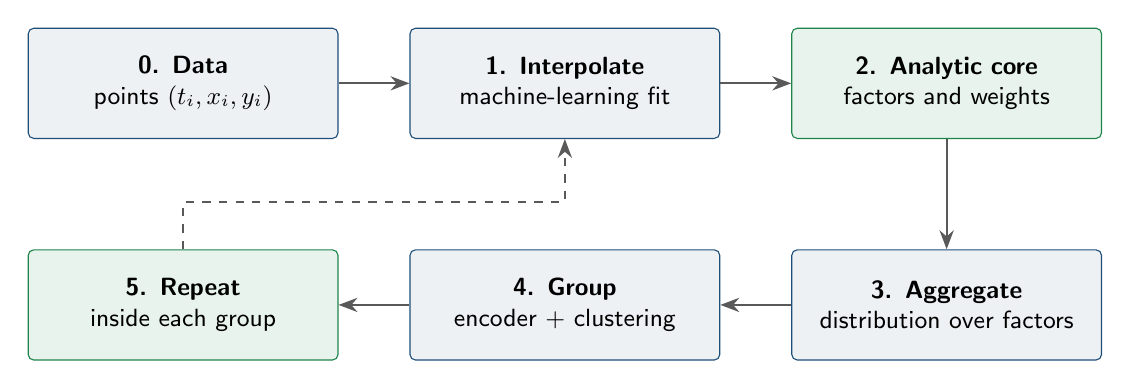
\begin{tikzpicture}[
  bx/.style={draw=cA,fill=cA!8,rounded corners=2pt,minimum height=14mm,text width=3.7cm,align=center,font=\small\sffamily},
  an/.style={draw=cC,fill=cC!10,rounded corners=2pt,minimum height=14mm,text width=3.7cm,align=center,font=\small\sffamily},
  ar/.style={-{Stealth[length=2.4mm]},thick,gray!70!black}]
\node[bx] (d) {\textbf{0. Data}\\ points $(t_i,x_i,y_i)$};
\node[bx,right=9mm of d] (i) {\textbf{1. Interpolate}\\ machine-learning fit};
\node[an,right=9mm of i] (f) {\textbf{2. Analytic core}\\ factors and weights};
\node[bx,below=14mm of f] (h) {\textbf{3. Aggregate}\\ distribution over factors};
\node[bx,left=9mm of h] (g) {\textbf{4. Group}\\ encoder $+$ clustering};
\node[an,left=9mm of g] (o) {\textbf{5. Repeat}\\ inside each group};
\draw[ar] (d)--(i); \draw[ar] (i)--(f); \draw[ar] (f)--(h); \draw[ar] (h)--(g); \draw[ar] (g)--(o);
\draw[ar,dashed] (o.north) -- ++(0,6mm) -| (i.south);
\end{tikzpicture}
\caption{The pipeline. Green boxes are the exact mathematical parts (already built); blue boxes are the machine-learning parts (to be designed). The dashed arrow is the loop: each group becomes a new data set.}
\label{fig:pipe}
\end{figure}

\begin{enumerate}[leftmargin=*]
\item \textbf{Interpolate.} A learning algorithm fits a smooth function to the data. Because data are finite, it returns not one function but \emph{many plausible ones, each with a probability}.
\item \textbf{Analytic core.} Each plausible function is handed to my algorithm. It spits out the factors that function contains and how much of the function each factor carries.
\item \textbf{Aggregate.} Add everything up, weighting by probability: we obtain a distribution (``transport appears with weight $0.7\pm0.1$, diffusion with $0.3\pm0.1$'').
\item \textbf{Group.} Use this distribution to \emph{set the parameters} of a standard grouping method (how many groups, how spread out) and cut the data into groups, so that each group ideally ``sounds like one instrument''.
\item \textbf{Repeat inside every group.} If the grouping was good, each group contains one (at most two) factors, and the tangle number is tiny. If not, regroup. When all groups are clean, the factors rebuild the equation.
\end{enumerate}

\subsubsection*{A tiny example, start to finish}
Suppose the (hidden) truth is
\[
u(t,x)\;=\;0.7\,e^{-(x-t)^2}\;+\;0.3\,e^{-t}\cos x .
\]
The first piece is a bump that \emph{travels} to the right with speed $1$. The second is a wave that \emph{spreads and fades}. We only see noisy samples of $u$.
\begin{itemize}[nosep]
\item \textbf{Step 1} returns many smooth curves close to $u$, each with a probability.
\item \textbf{Step 2}, applied to each curve, finds the two factors
\[
Q_1=\partial_t+\partial_x\ \ (\text{transport}),\qquad Q_2=\partial_t-\partial_x^2\ \ (\text{diffusion}),
\]
and the pieces $u_1=0.7\,e^{-(x-t)^2}$ and $u_2=0.3\,e^{-t}\cos x$.
\item \textbf{Step 3} reports: transport $\approx 70\,\%$, diffusion $\approx 30\,\%$, with their spread.
\item \textbf{Step 4} uses ``two main factors'' to choose ``two groups'' and cuts the data accordingly.
\item \textbf{Step 5} re-analyses each group alone: the first group shows only transport, the second only diffusion, and the tangle number is close to zero in both. We stop and write down the equation.
\end{itemize}

%==========================================================
\subsection*{Part II --- A little mathematics}
\addcontentsline{toc}{section}{Part II --- A little mathematics}

\begin{notebox}{Scope}
Everything in the analytic core assumes \textbf{exact} data and a \textbf{linear equation with constant coefficients}. This is the part I have worked out with complete proofs. The statistical wrapper (Sections~\ref{sec:wrap}--\ref{sec:loop}) is a \emph{proposal}: this is where I need you.
\end{notebox}

\subsubsection{Setting}
Let $u(t,x)$ be defined on a bounded region $\Omega\subset\R^2$. It satisfies a linear equation with constant coefficients $P(\partial_t,\partial_x)\,u=0$ that is \emph{not} known. Replacing $\partial_t\to\tau$, $\partial_x\to\xi$ turns an operator into a polynomial, its \emph{symbol}. Polynomials factor, and the factors are our ``instruments'':
\[
P=Q_1Q_2\cdots Q_N .
\]
For the example above, $P=(\tau+\xi)(\tau-\xi^2)$.

\subsubsection{The analytic core (exact data)}\label{sec:core}

\paragraph{(i) Factors generate components.}
If the $Q_j$ are pairwise coprime and $\Omega$ is simply connected, every solution splits as
\[
u=\sum_{j=1}^{N}u_j,\qquad Q_j(\partial)\,u_j=0 .
\]
The split is unique up to a finite-dimensional space of exponential-polynomials, of dimension
\[
\delta(P)=\sum_{i<j}\dim_{\mathbb C}\,\mathbb C[\tau,\xi]\big/(Q_i,Q_j).
\]
(This is the Chinese Remainder Theorem in two variables; the ambiguity is a few exponentials, not a function.) \emph{Splitting by additive terms of $P$ instead of factors is false in general.}

\paragraph{(ii) Evolution factors have an explicit projector.}
If $Q_j=\partial_t-a_j(\partial_x)$ with distinct $a_j$, then applying all the other factors kills every other component:
\[
\prod_{k\ne j}\big(\partial_t-a_k(\partial_x)\big)\,u\;=\;\prod_{k\ne j}\big(a_j-a_k\big)(\partial_x)\,u_j .
\]
So $u_j$ is recovered by ``dividing'' by $\prod_{k\ne j}(a_j-a_k)(\partial_x)$, up to its kernel (this is the finite ambiguity). In the example, $a_1=-\partial_x$, $a_2=\partial_x^2$, and the division is by $-\partial_x(1+\partial_x)$, whose kernel $\mathrm{span}\{1,e^{-x}\}$ has dimension $2=\delta(P)$.

\paragraph{(iii) Terms inside a factor.}
A single factor $\partial_t-a(\partial_x)$ may itself be a sum of \emph{terms}, $a=\sum_n a_n$ (advection, diffusion, \dots). In Fourier variables $\hat u(t,\kappa)=\int u\,e^{-i\kappa x}\dd x$,
\[
\log\hat u(t,\kappa)\;=\;\log\hat u_0(\kappa)\;+\;t\sum_{n=1}^{N} a_n(\kappa),
\]
which is \emph{linear in the terms}: they are read off by regression on monomials in $\kappa$. For advection--diffusion $u_t=-cu_x+Du_{xx}$ one finds $a_1=-ic\kappa$, $a_2=-D\kappa^2$.

\paragraph{(iv) The interaction term.}
Let $S_n(t)=e^{tA_n}$ be the evolution generated by term $n$ alone and $\Delta_n=S_n(t)-\mathrm{Id}$. Define the part of $u$ that \emph{no single term explains}:
\[
\Eint\;=\;u(t)-u_0-\sum_{n=1}^N\big(S_n(t)u_0-u_0\big).
\]
For commuting terms (constant coefficients) it has the exact closed form
\[
\Eint=\Big[\prod_{n=1}^N(\mathrm{Id}+\Delta_n)-\mathrm{Id}-\sum_{n=1}^N\Delta_n\Big]u_0,
\]
or, in Fourier variables,
\[
\widehat{\Eint}(t,\kappa)=\Big[\prod_n e^{ta_n(\kappa)}-1-\sum_n\big(e^{ta_n(\kappa)}-1\big)\Big]\hat u_0(\kappa).
\]
Its value costs $O(N)$ operations (never expand the product). Two properties give the diagnostic its meaning: $\Eint=0$ if only one term acts ($N=1$), and for $N=2$ we have $\Eint=\Delta_1\Delta_2u_0$, the \emph{product} of the two single-term effects. For advection--diffusion,
\[
\frac{|\widehat{\Eint}|}{|\hat u_0|}=\big|(e^{-ic\kappa t}-1)(e^{-D\kappa^2 t}-1)\big|\le 2 .
\]

\begin{notebox}{Two different notions of ``tangle''}
It is useful to keep two quantities apart. \textbf{Between factors}: how hard is it to separate $u_1$ from $u_2$? For two factors this is measured by the Friedrichs cosine $c_F$ (the cosine of the smallest angle between $\ker Q_1$ and $\ker Q_2$, modulo their intersection): $c_F\to1$ means the components are nearly indistinguishable. \textbf{Inside a factor}: how much do its terms interact? This is $\Eint$. A good grouping makes both small. A single factor with two real terms (advection--diffusion) is a legitimate output even though $\Eint\neq0$: there $\Eint$ is information, not an error.
\end{notebox}

\subsubsection{Statistical wrapper (proposal)}\label{sec:wrap}

\paragraph{Step 1: a distribution of interpolants.}
The interpolation step returns a weighted family
\[
\big\{(\hat u_s,\pi_s)\big\}_{s=1}^S,\qquad \pi_s\ge0,\quad \sum_s\pi_s=1,
\]
for instance posterior samples from a Gaussian process, a Bayesian neural network, or an ensemble. The \emph{basis functions} of this fit are the object of Question~1: they may be (a) solutions of known operators (e.g.\ $e^{\lambda t+i\kappa x}$, travelling waves), so each basis function maps directly to a factor, or (b) generic functions (networks, kernels), in which case the analytic core must extract factors from the fitted function itself.

\paragraph{Step 2: analytic core, sample by sample.}
For each $\hat u_s$ the core returns factors $Q^{(s)}_j$ (with coefficient vectors $\theta^{(s)}_j$ in the space of operator coefficients) and components $u^{(s)}_j$. Define the weight of a factor as its share of the signal,
\[
w^{(s)}_j=\frac{\|u^{(s)}_j\|}{\sum_k\|u^{(s)}_k\|},
\]
choosing the minimum-norm representative to fix the finite ambiguity. If $\hat u_s$ is a linear combination of basis functions, this is simply the (normalised) coefficient mass attached to each factor, as in the toy example, where a coefficient of $0.5$ on a basis function sends weight $0.5$ to its factor.

\paragraph{Step 3: distribution over factors.}
The result of aggregation is a weighted cloud in coefficient space,
\[
\mathcal W\;=\;\sum_{s=1}^{S}\ \pi_s\sum_{j}w^{(s)}_j\ \delta_{\theta^{(s)}_j}.
\]
From $\mathcal W$ we read: the dominant factors (modes of the cloud) with their total mass $W_j$, their means $\bar\theta_j$ and covariances $\Sigma_j$; the \emph{effective number of factors}
\[
k_{\mathrm{eff}}=\exp\Big(-\sum_j W_j\log W_j\Big);
\]
and the co-occurrence of factors across samples (which factors appear together), plus the average interaction and the average separability,
\[
\bar\rho=\sum_s\pi_s\,\frac{\|\Eint(\hat u_s)\|}{\|\hat u_s-u_0\|},\qquad \bar c_F=\sum_s\pi_s\,c_F\big(\hat u_s\big).
\]

\paragraph{Step 4: using $\mathcal W$ to set the clustering.}
My proposal (to be criticised): the number of groups is $k=\lceil k_{\mathrm{eff}}\rceil$; the initial centres are the $\bar\theta_j$; the within-group variances are the $\Sigma_j$; the encoder dimension is of the order of the number of dominant factors, and the encoder is any of PCA, SVD, an autoencoder; the grouping algorithm is any of $k$-means, a Gaussian mixture, spectral clustering.

Two natural \emph{notions of group} appear in the analytic theory, and one could use either, even different ones at different stages: (a) a group is a \emph{kernel} $\ker Q_j$, i.e.\ functions annihilated by a factor (``multiplication by the operator'' picture); (b) a group is a \emph{flow family} $\{e^{tA_n}u_0\}$, i.e.\ what a term does alone (``exponential of the operator'' picture).

\subsubsection{The loop}\label{sec:loop}
\begin{ideabox}[title={Algorithm (outer loop)}]
\begin{enumerate}[nosep,leftmargin=*]
\item Fit the dataset $\mathcal D$ $\Rightarrow$ $\{(\hat u_s,\pi_s)\}$.
\item Run the analytic core on every $\hat u_s$ $\Rightarrow$ $\mathcal W$ and the statistics $k_{\mathrm{eff}},\ \bar\rho,\ \bar c_F$.
\item If the groups are \emph{clean} (each has $\le2$ factors, $\bar\rho<\varepsilon_1$, $\bar c_F<\varepsilon_2$), \textbf{stop}.
\item Otherwise set the encoder and clustering parameters from $\mathcal W$, split $\mathcal D$ into $\mathcal D_1,\dots,\mathcal D_k$, and \textbf{recurse} on each $\mathcal D_g$.
\item Reconstruct the equation from the surviving factors, with their probabilities.
\end{enumerate}
\end{ideabox}

\subsubsection{What is known and what is not}
\begin{table}[!htb]
\centering\small
\begin{tabular}{@{}p{5.2cm}p{3.2cm}p{5.5cm}@{}}
\toprule
Statement & Status & Remark\\\midrule
Factors give components; ambiguity $\delta(P)$ & proved (exact data) & simply connected $\Omega$; fails otherwise\\
Components are in $H^m$ for all $u$ & iff sum of kernels closed & needs a gap condition ($\gamma_N>0$); not automatic\\
Closed formula for $\Eint$, cost $O(N)$ & proved & constant coefficients (commuting terms)\\
$u_0\mapsto\Eint$ continuous in $H^m$ & \textbf{false} & stability under noise is a real issue\\
Finite data certify the equation & \textbf{impossible} & no finite certificate; black box impossible\\
Nonlinear extension & partial & Burgers: closed form before the shock\\
Dictionary identification, nonlinear & exact modulo differential consequences & a countable dictionary cannot identify everything\\
Statistical wrapper (II.3--II.4) & \textbf{proposal} & no convergence or noise-robustness theory\\
\bottomrule
\end{tabular}
\caption{What the analytic theory guarantees, and what is still open.}
\end{table}

The last rows are the reason for this note: the analytic core is exact but fragile under noise, and the statistical wrapper is exactly the mechanism that could make it usable.

%==========================================================
\subsection*{Part III --- Questions for you}
\addcontentsline{toc}{section}{Part III --- Questions for you}

\begin{askbox}{Q1 --- Must the basis functions be chosen in advance?}
If the interpolation uses basis functions that solve known equations (exponentials for constant coefficients, travelling waves for transport, Bessel or Airy functions for others), then the method is easy to implement, but \emph{it can only discover equations whose building blocks are in the list}. For example, if there is no transport-type basis function, a transport equation may be misidentified. A fully generic fit (neural network, kernel method, Gaussian process) avoids the choice, but then the analytic core must extract factors from a function with no built-in structure.\\[3pt]
\textbf{Is there a standard way to avoid committing to a basis in advance} (e.g.\ learning the basis, a nonparametric fit followed by Fourier- or jet-based extraction, a hierarchy of dictionaries), \textbf{and what does one lose in doing so?}\\[3pt]
\emph{Relevant fact from the analytic side:} no countable dictionary identifies everything exactly, and with a fixed dictionary one only recovers an equation modulo its differential consequences. So the question is not purely technical.
\end{askbox}

\begin{askbox}{Q2 --- Designing the outer structure}
I constructed the analytic core. I would like advice on everything around it:
\begin{enumerate}[nosep,leftmargin=*]
\item \textbf{Loop and stopping rule.} Is ``recurse until each group is clean'' sensible? How to choose the thresholds $\varepsilon_1,\varepsilon_2$?
\item \textbf{Parameter estimation.} Is deriving $k$, the centres and the variances from the factor distribution $\mathcal W$ reasonable? Would you instead learn them jointly (end-to-end, EM, variational), with the analytic core as a differentiable layer?
\item \textbf{Choice of encoder and clustering.} PCA, SVD, an autoencoder; $k$-means, Gaussian mixtures, spectral methods. Which are appropriate when the ``clusters'' are defined by a differential structure rather than by distance?
\item \textbf{Uncertainty.} How should the probability from the interpolation step be propagated through a non-linear, possibly discontinuous map (the interaction term is not continuous in $H^m$)?
\item \textbf{Noise and validation.} What would a convincing experiment look like (synthetic data from known equations first)? Which baselines (SINDy, PDE-FIND, neural PDE learners) should it be compared against?
\end{enumerate}
\end{askbox}

\paragraph{Proposed way of working.}
Start with synthetic data from two or three known linear equations (transport $+$ diffusion mixtures like the example above). I supply the analytic core as a routine, together with the written proofs of the properties above; you design the outer structure and the experiments. The first deliverable would be the reconstructed factor distribution on those synthetic cases, compared against known ground truth.



% ---- end sections/note.tex


% embedded bibliography (generated by BibTeX from the .bib files of the earlier multi-file version)
\begin{thebibliography}{1}

\bibitem{AngEtAl24}
Anastasios~N. Angelopoulos, Stephen Bates, Adam Fisch, Lihua Lei, and Tal
  Schuster.
\newblock Conformal risk control.
\newblock In {\em International Conference on Learning Representations}, 2024.
\newblock arXiv:2208.02814.

\bibitem{BarEtAl21}
Rina~Foygel Barber, Emmanuel~J. Cand{\`e}s, Aaditya Ramdas, and Ryan~J.
  Tibshirani.
\newblock Predictive inference with the jackknife+.
\newblock {\em The Annals of Statistics}, 49(1):486--507, 2021.

\bibitem{Fri01}
Jerome~H. Friedman.
\newblock Greedy function approximation: a gradient boosting machine.
\newblock {\em The Annals of Statistics}, 29(5):1189--1232, 2001.

\bibitem{RasWil06}
Carl~Edward Rasmussen and Christopher K.~I. Williams.
\newblock {\em Gaussian Processes for Machine Learning}.
\newblock MIT Press, Cambridge, MA, 2006.

\end{thebibliography}

\end{document}
